%\documentclass[capnocolon,titlechinese]{ustcthesis}
\documentclass[oneside,openany,capnocolon,titlechinese]{ustcthesis}
\usepackage{metalogo}
%\usepackage{floatrow}
\usepackage{verbatim}

% 设置图形文件的搜索路径
\graphicspath{{chapter/}{figures/}}
\begin{document}
%%%%%%%%%%%%%%%%%%%%%%%%%%%%%%
%% 封面部分
%%%%%%%%%%%%%%%%%%%%%%%%%%%%%%
  % 中文封面内容
  %如果使用\makeseparatetitle命令生成扉页,当中文标题过长时可以将多余的标题放在\titletail{}中
  \title{基于图像通道相关性的}
  \titletail{彩色图像可逆隐藏算法研究}
  \entitle{Reversible Data Hiding Method for Color Image Based on Inter-Channel Correlation}
  %全角空格可以正常输出
  \author{马国力}
  \enauthor{Guoli Ma}
  \department{信息学院\ 信息安全专业}
  \No{PB10210141}
  \tutor{张卫明\ 教授}
  \entutor{Prof.Weiming Zhang}
  \cntime{二〇一四年五月}
  \entime{May,2014}
  %生成封面(制本厂要求的格式)
  \makecover
  % 扉页形式
  %生成中英文合并的扉页
  \maketitle
  %生成中英文分开的扉页
  \makeseparatetitle

%%%%%%%%%%%%%%%%%%%%%%%%%%%%%%
%% 前言部分
%%%%%%%%%%%%%%%%%%%%%%%%%%%%%%
\frontmatter

  % 致谢
  
\begin{thankspage}
首先我要感谢俞能海教授。俞老师是我的实验室导师,也是我们的系主任。无论是在学业
还是在生活上,我们都受到了俞老师莫大的关怀和帮助。他不仅对我们的科研提出了很多
宝贵的指导意见,还关注我们的个人成长,处处为同学着想,教会了我们很多为人处世的
道理。同时,在生活上俞老师随和可亲,为学生的发展尽心尽责。每次同俞老师的交流都
让我受益良多。我会将您的教诲作为我前行道路上的明灯。
\par
我还要感谢我的导师张卫明老师。从刚入实验室时指导我调研、阅读文献,到如今毕业设计
的选题、算法设计、实验验证,以及论文的撰写,张老师严肃的科学态度,严谨的治学精神,
精益求精的工作作风一直在深深的感染和鼓励着我。通过张老师组织的每周的讨论班,我不
仅能够对工作做出总结和安排,还阅读和学习了大量的新文献,这对我毕设的工作起了关键的
作用。而当毕设遇到困难时,张老师也会耐心的给出指导。感谢您这两年来给予我的无私付
出和教导。
\par
另外,我要特别感谢北京大学的彭飞师兄和李小龙老师,感谢你们的论文和代码,它们
奠定了我毕业设计的基础,也为我的课题提供了很多的便利。
\par
此外,我还要感谢实验室的师兄师姐们,特别感谢胡校成师兄、姚远志师兄,感谢他们在
毕设过程中给予我的帮助。感谢一同在实验室奋斗的周文柏、管成杰、刘润东、
盛化龙、张卓、魏尧和南杰慧同学和我的室友张卓、汤琦、孙骁永,感谢你们给我的
生活带来的快乐。感谢梁爽童鞋三年来的陪伴。
\par
最后,感谢赋予我生命和养育我成人的父亲母亲,感谢他们二十多年为我操劳和付出,祝福
他们永远健康、幸福!
\end{thankspage}

  % 目录

  \tableofcontents
  % 摘要
  
\begin{cnabstract}
信息隐藏技术是一种将数据嵌入到各种载体中的技术,在现实生活中得到了广泛的应用。而
可逆信息隐藏则是信息隐藏技术的一个特别的分支,它不仅关注要嵌入的用户数据,更关注
载体本身。它要求载体在提取出被嵌入的消息后,仍然能被完整的恢复。这就对消息的嵌入
方式提出了更高的要求。而正是由于可逆信息隐藏的这种特性,它在医学图像保护、载体篡
改认证和恢复、数字媒体版权保护中得到了广泛的应用。
\par
可逆隐藏技术在过去十几年间得到了长足的发展。学者们针对数字图像、视频、音频等载体
提出了各种各样的可逆隐藏算法。其中研究的热点集中在数字灰度图像邻域。但是在现实生
活中,使用最多的是彩色图像。现阶段针对彩色图像的可逆隐藏文献很少,针对这种情况,
本论文从彩色图像的通道相关性出发,对彩色图像的可逆隐藏技术进行了研究,提出了一种
针对彩色图像的可逆隐藏算法。
\par
算法首先结合彩色图像的通道相关性,使用了一种利用通道内预测误差进行通道间二次预测
的新预测方法,实验表明,这种预测方法能比以往算法得到更陡峭、熵更小的预测误差直方
图。随后,论文介绍了一种新的排序算法。同以往排序算法不同,该算法通过对当前像素的
预测误差概率分布进行预测,兼顾了邻域的像素的预测差值和方差,能更好的反映像素的纹
理复杂度。最后通过实验比较发现,所提出的算法在嵌入容量和图像质量上比以往算法有了
一定的提升。

\cnkeywords{可逆信息隐藏,通道相关性,图像预测}
\end{cnabstract}


\begin{abstract}
Information hiding is a widely used technology that embeds data into different 
digital carriers. Reversible information hiding, as a special branch of         
information hiding, it is not only concerned about the user's embedding data,   
but also pay attention to the carriers themselves. It requires the carriers to  
be completely recovered after extracting the embedded message. This will put    
forward higher requirements for the ways of data embedding. But because of this 
feature, reversible information hiding has been widely used in medical image    
protection, authentication and tamper carrier recovery, and digital media      
copyright protection.                                                           
\par
In the last ten years, reversible hiding has been considerably developed.      
Scholars have proposed a variety of reversible hiding algorithms for digital    
images, digital videos, audios, and other carriers. And the hot spot is         
concentrated on digital gray-scale images. But in real life, it is the color    
images that are widely used. In recent days, reversible data hiding for color   
images is a rarely studied topic. So this thesis will focus on reversible data
hiding method for color images. Based on the inter-channel correlation of color
image, a novel inter-channel prediction method is examined and a corresponding
reversible data hiding algorithm is proposed.           
\par
In the proposed method, the prediction error is obtained by an inter-channel   
secondary prediction using the prediction errors of two independent             
channels. Experiments show that this prediction method can produce shaper       
Prediction-Error-Histogram (PEH). Then, we will introduce a new pixel-sorting   
algorithm that will make predictions for the probability distribution of        
prediction error of current pixel. It can utilize both differences and the         
prediction variances of neighborhood pixels. So it will reflect the texture
complexity of current pixel better. Finally, as the experiments demonstrated,
the proposed algorithm has some improvement over the previous algorithm on both
the embedding capacity and image quality.

\keywords{Reversible Data Hiding, Inter-Channel Correlation, Image Prediction}
\end{abstract}



%%%%%%%%%%%%%%%%%%%%%%%%%%%%%%
%% 正文部分
%%%%%%%%%%%%%%%%%%%%%%%%%%%%%%
\mainmatter
  \chapter{绪论}
\label{chap:introduction}

\section{论文研究背景及应用}
\label{s:background}
信息隐藏技术是信息安全领域中一个重要的研究方向,它是一种将数据嵌入到各种载体中的
技术,它被大量应用在隐秘通信、篡改认证和版权保护中。狭义的信息隐藏技术,被称为隐
写术(Steganography)。隐写术将秘密消息隐藏在一些公开传输的媒介中,利用公开媒介
来掩护消息的传输,主要关注通信的隐蔽性。隐写术要求对载体进行微量的随机修改,以防
止被隐藏的消息被通信对端以外的第三方发现。与隐写术相对的技术称为隐写分析技术
(Steganalysis)。它通过对公开传输媒介的统计特征进行分析,以判断媒介中是否被隐藏
了消息。对隐写、隐写分析的研究有助于对非法活动进行监控,对维护社会稳定,保护国家
及人民安全有着至关重要的作用。
\par
但是隐写术并不关心对载体的保护,当秘密消息被提取后,载体通常不能被完美地恢复。而
这种情况在一些应用中是不允许的,例如以医疗、军事图像为载体的信息隐藏,这些应用对
图像质量有着相当高的要求,即使微小的改变也不能被接受。因此,学者们提出了可逆的信
息隐藏(Reversible Data Hiding,RDH)技术。可逆信息隐藏技术不仅关注秘密消息,同
时也关注对载体本身的保护。通过特殊的嵌入算法,载体的原始信息被保护起来,当消息被
提取之后,原始信息能够被可逆的恢复。同隐写不同的是,大多数可逆隐藏算法并不关注
消息本身的隐蔽性,它不被用来进行隐蔽通信。
\par
由于可逆隐藏技术载体可恢复的特点,它在现实生活中得到了广泛的应用,具体应用如下:
\par
%\vspace{-2mm}
\begin{itemize}
  \setlength{\parindent}{2em}
  \vspace{-3mm}
  \item \textbf{信息管理}
  \vspace{-2mm}
  \par
  随着互联网的发展,网络上的数据量日益增大,如何对如此庞大的数据进行管理是一个
  关键的问题。文献\cite{hwang2010trusted}中,作者基于可逆信息隐藏,提出了一种
  云计算的保障机制。作者在云端服务器存储的用户数据中嵌入了对应的用户信息,节省
  了大量的数据库空间。另外,在医院,常常将患者的个人隐私信息通过可逆隐藏技术
  嵌入到医学图像当中,这样既可以起到隐私保护的目的,又可以对大量图像进行管理。
  \par
  \vspace{-3mm}
  \item \textbf{完整性认证}
  \vspace{-2mm}
  \par
  PS、Audition等数字媒体处理软件的出现使得网络上出现了众多虚假的照片、音频,使
  人难辨真伪。而利用信息隐藏,可以在载体中嵌入与载体高度相关的哈希特征值,或者
  载体的参考信息(Reference Value)。这样当使用者得到这些载体时,他们可以重新
  计算载体哈希特征,与其中嵌入的特征进行比较,以判断载体是否被修改,以及在什么
  位置被修改,甚至利用参考信息,恢复出原始载体的部分或全部信息。而由于信息嵌入
  的可逆性,当载体没有被破坏时,原始载体可以被完美恢复。
  \par
  \vspace{-3mm}
  \item \textbf{版权信息保护}
  \vspace{-2mm}
  \par
  被用于版权信息保护的信息隐藏技术通常又被称为数字水印(Digital Watermarking)
  技术或者数字指纹技术(Digital Fingerprint)。水印技术通过将商业产品标识,如
  特征码,商标等信息嵌入到产品中,指示产品的版权归属。而数字指纹技术则常常将
  已授权用户的相关信息嵌入到产品当中,通过检测盗版产品中的用户相关信息就可以
  追查到盗版源头。这种技术同人类指纹有着相似的作用,因此被称为数字指纹,以防
  止合法用户未经许可散播产品给未授权用户。\\
\end{itemize}



\section{可逆信息隐藏技术的分类}
\label{s:type_application_reversible_data_hiding}
\begin{figure}[!ht]
\centering 
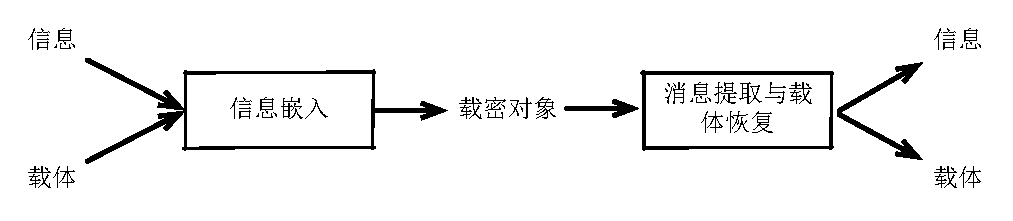
\includegraphics[width=0.7\textwidth]{figures/reversible_framework.eps}
\caption{可逆信息隐藏的一般框架}
\label{fig:revers_framework}
\end{figure}
自从可逆隐藏技术提出以来,这个领域的研究就非常的活跃,学者们提出了各种各样有效
的算法。图\ref{fig:revers_framework}是可逆信息隐藏系统的一般框架,基本所有的算
法有符合这个框架。在``信息嵌入''模块,秘密信息被嵌入载体对象中,得到载密对象。接
收方利用``信息提取与载体恢复''算法,从载密对象中提取出秘密信息,并恢复出原始载体。
一般认为,信息嵌入过程不能对载体对象造成明显的修改。现有的可逆隐藏算法根据它们
的载体、稳健性等方面的差异,可以分为不同的类型。\\
\vspace{-8mm}
\begin{itemize}
  \setlength{\parindent}{2em}
  \vspace{-2.5mm}
  \item \textbf{以载体类型分类}\\
  \vspace{-10mm}
  \begin{itemize}
    \setlength{\parindent}{2em}
    \item[*] \textbf{基于空域图像}
    \vspace{-1mm}
    \par
    基于空域图像的可逆隐藏算法得到了广泛的研究,大多数算法都以8比特灰度图像为载
    体,对像素进行一定的修改,以达到可逆隐藏的目的。本质来说,针对空域图像的可逆
    隐藏算法同可逆压缩算法类似,都需要找到像素间的相关性,通过可逆手法去除
    像素相关以腾出空间嵌入秘密信息。不同的算法在不同的嵌入率下有着不同的表现,有
    的算法针对小嵌入率进行特殊的改进,以最大限度的提高图像质量;有的算法则注重嵌
    入容量,期望在可以容忍的图像质量下尽可能提高嵌入率。
    \par
    \vspace{-2mm}
    \item[*] \textbf{基于JPEG图像}
    \vspace{-1mm}
    \par
    JPEG作为当今最为流行的图像压缩算法,在可逆隐藏中也同样得到了深入关注。JPEG压
    缩基于DCT变换,而针对JPEG图像的可逆压缩算法也主要集中在对DCT变换系数,量化表
    等方面。本质上,DCT变换也是一种去除图像块冗余的算法,因此JPEG图像天然地使用
    于做可逆隐藏。一种常见的算法是利用每个图像块DCT系数中的0系数,例如可以寻找特
    殊的全零模式,因此这样的每个‘0’模式都可以被用来嵌入1比特信息。
    \par
    \vspace{-2mm}
    \item[*] \textbf{基于其他载体}
    \vspace{-1mm}
    \par
    随着可逆隐藏技术的不断发展,学者们不在将眼光局限在图像领域,他们尝试将可逆隐
    藏算法应用到更广泛的载体中。例如一些一维信号如音频、心电图。还有一些文献则将
    可逆隐藏的思想应用到了视频领域\cite{xu2014improved},提出了针对H.264视频的视
    频容错编码方法。文献将可逆隐藏技术同冗余片进行结合,能很有效的保障移动通信中
    的视频质量。\\
  \end{itemize}
  \vspace{-11mm}
  \item \textbf{以稳健性分类}\\
  \vspace{-10mm}
  \begin{itemize}
    \setlength{\parindent}{2em}
    \item[*] \textbf{脆弱水印}
    \vspace{-1mm}
    \par
    所谓脆弱水印,是一种当载体遭到修改后很容易被改变或毁掉的印记。由此可见,脆弱
    水印并不适合进行版权保护等工作,因为攻击者很容易就可以破坏载体中的水印。然而
    正是脆弱水印的这种对修改的敏感性,使得其被广泛的应用于图像鉴别、图像完整性认
    证等应用中。而同签名技术相比,脆弱水印被嵌入到了载体中而不需要任何的附加信息,
    节省了通信成本。另一方面,脆弱水印能够更加精确地定位篡改位置,从而使得重传成
    本进一步降低。
    \par
    \vspace{-2mm}
    \item[*] \textbf{稳健水印}
    \vspace{-1mm}
    \par
    同脆弱水印对修改的敏感性不同,稳健水印要求载体中的水印信息在载体遭到一定的攻
    击(如压缩、加噪、滤波)时,仍然不能收到破坏,能够被提取出来完成认证工作。稳
    健水印的这种特性可以被用来进行版权认证等工作。另外,稳健水印的一些特性可以用
    在隐写等隐蔽通信的应用中。例如利用一些水印的抗打印、抗拍照等特性,可以将秘密
    信息隐藏到照片中,利用照片传递来进行秘密通信。\\
  \end{itemize}
\end{itemize}



\section{本文研究内容及论文结构}
\label{s:contribution_of_this_thesis}
如前所述,当前信息隐藏研究重点主要集中在灰度图像上,不论是狭义上的隐写技术,还
是可逆隐藏技术,针对灰度图像的算法在过去得到了广泛的研究。然而在现实生活中,使
用最多的却是彩色图像,针对彩色图像的可逆隐藏算法将是未来的研究热点。
\par
同灰度图像不同,彩色图像有R、G、B三个通道,这三个通道间存在着高度的相关性,这些
相关性为可逆隐藏提供了良好的条件。本论文中提出了一种简单的基于彩色图像通道相关性
的可逆隐藏算法。论文中发现,当通过通道内的预测去除通道内相关性之后,三个通道的预
测误差的大小和结构基本相同。据此,论文提出了采用通道间进行二阶预测的算法。另外,
论文使用了一种新的排序算法:利用像素的邻域像素对预测误差的分布参数进行预测。利用
论文提出的算法,彩色图像的可逆隐藏算法的嵌入容量和图像质量得到了一定程度的提升。
\par
本论文一共分为四章,各章的内容如下:
\par
第一章主要介绍论文的研究背景,简单介绍了信息隐藏技术,对可逆隐藏技术进行了分类,
并简单介绍了隐写技术、可逆信息隐藏技术的分类和应用,简单陈述了论文的主要内容和
论文结构。
\par
第二章对主流的针对灰度空域图像的常用可逆隐藏算法,以及算法中常用的排序技术进行
了详细的介绍,算法包括基于可逆隐藏的算法,基于直方图平移、差值扩展、预测误差扩
展的算法,基于整数变换的算法等,最后则介绍了一种最新的针对彩色图像的可逆隐藏算
法。
\par
第三章则详细介绍分析了本论文提出的基于彩色图像通道相关性的算法。本章主要从预测
算法、排序算法、完整的嵌入算法及流程图以及实验结果四个角度对算法进行详细的展示。
\par
第四章将对本文的工作做出一定的总结,分析现有工作的不足之处,并对可能的后续工作
进行了展望。\\

  \chapter{常见可逆隐藏算法介绍}
\label{chap:related_intro}
当今可逆隐藏领域的研究主要以图像为载体,虽然也有针对其他载体的可逆隐藏算法,但是
最成熟的算法仍然集中在灰度图像领域,例如:基于可逆压缩的
算法\cite{fridrich2001invertible,celik2005lossless}、基于直
方图平移\cite{ni2006reversible,lee2006reversiblee,li2013general}、差值
扩展\cite{tian2003reversible,alattar2003reversible,alattar2004reversible,alattar2004reversible}、
预测误差扩展的算法\cite{thodi2007expansion},基于整数变换的算法
\cite{coltuc2007very,chen2010reversible,wang2010efficient,peng2012adaptive},以
及能够较大程度上提升可逆隐藏效果的排序技术
\cite{kamstra2005reversible,sachnev2009reversible}本节将对灰度图像和
彩色图像的常用可逆隐藏算法进行详细的回顾和总结。



\section{灰度图像可逆隐藏算法}
\subsection{可逆压缩}
\begin{itemize}
  \setlength{\parindent}{2em}
  \vspace{-2mm}
  \item \textbf{早期基于可逆压缩算法}
    \vspace{-2mm}
    \par
    早期的可逆隐藏算法主要基于可逆压缩算法,而可逆隐藏的本质也可以归于可逆压缩领
    域。基于可逆压缩的可逆隐藏算法的本质是对载体图像的一个特征集$S$进行可逆压缩,
    利用压缩出的部分空间进行消息嵌入。嵌入的简单实现是将$S$换为其压缩形式$S_c$和
    消息$M$,因此最大的嵌入容量(Embedding Capacity, EC)为$S-S_c$。显然基于可逆
    压缩的算法效果取决于压缩算法和选取的特征集。
    \par
    2001年\cite{fridrich2001invertible},Fridrich提出的可逆隐藏算法通过对有最小
    冗余度的位平面(bit-plane with the minimum redundancy)进行压缩来获得空间。
    在他们的算法中,除非图像噪声很大,否则总是最低位平面被用来压缩和隐藏。同年
    \cite{fridrich2001invertible2},Fridrich针对JPEG图像提出了一种基于可逆隐藏的
    算法。该算法对变换域的每个块的固定位置提出其DCT系数,由于DCT变换的性质,这
    些系数构成一个有偏序列,进而可以利用可逆压缩为消息嵌入提供空间。
    \par
    文献\cite{celik2005lossless}中,Celik提出了一种广义LSB替换的算法,改进了
    Fridrich算法的性能。算法首先将图像分成不相交的小块,将块中每个像素对$L$取模
    后的余数序列进行无损压缩。将消息转换成$L$进制后填充压缩出来的空间,再反变换
    为灰度值。这种算法将消息嵌入到每个像素对$L$取模的余数上,通过采用$L$个码元,
    而不是Fridrich算法的2个,提高了嵌入容量。
    \par
    早期基于可逆隐藏的算法最大的问题在于其嵌入容量过小。考虑一个8比特灰度图像,
    每个像素的取值范围为$[0, 255]$,而在基于可逆压缩的算法中,要将一个8比特整数
    映射到一个二元或者$L$元整数,在映射像集进行嵌入。这样载体中大量的可用嵌入空
    间没有得到利用,实际嵌入率为0.1 bpp(bit per pixel,每比特嵌入容量)左右,限
    制了该算法的发展和应用。\\
  \vspace{-10mm}
  \item \textbf{近期基于可逆压缩算法}
    \vspace{-2mm}
    \par
    如前所述,可逆隐藏本质上可以归于可逆压缩,那么基于信息论,可逆隐藏就可以抽
    象出这样一种问题:对于给定的失真界限,一个特定的载体图像的嵌入容量上界是什
    么?对于这个问题,Kalker和Willems在文献\cite{kalker2002capacity}中给出了解
    答。他们认为可逆隐藏问题可以看成一种特殊的率失真问题,在给定失真界限为
    $\Delta$时,率失真函数,即嵌入率上界为:$\rho_{rev}=maximize\{H(Y)\}-H(X)$,
    其中$X$,$Y$分别表示载体和载密信号,而转移概率矩阵为$P_{Y|X}=(y|x)$,即载体
    信号$x$修改为载密信号$y$的概率,应满足失真界$\sum_{x,y}P_X(x)P_{Y|X}(y|x)
    D(x,y)\le\Delta$,其中$D(x,y)$通常定义为平方失真$(x-y)^2$。
    \par
    根据此理论,学者们提出了一些能够达到理论率失真界限的,基于可逆压缩的可逆隐藏
    算法,而所有这些算法都可以看成是文献\cite{kalker2002capacity}中递归编码构造
    (recursive code construction)的改进。下面通过递归直方图修改(recursive 
    histogram modification, RHM),对算法做简单介绍。
    \par
    RHM首先估计最优转移概率$P_{Y|X}(y|x)$和$P_{X|Y}(x|y)$,然后将载体图像分成不
    相交的块,利用一种熵编码的压缩和解压缩算法,基于最优转移概率,将消息递归地通
    过修改每个块的直方图的方式嵌入到每个块中。以一块为例,设块$\textbf{x}=(x_1,
    \cdots,x_K)$满足概率分布$P_X$,基于转移概率$P_{Y|X}(y|x)$,将$S$比特消息
    $\textbf{m}=(m_1,\cdots,m_S)$解压缩为载密序列$\textbf{y}=(y_1,\cdots,y_K)$并
    用$\textbf{y}$替换$\textbf{x}$。由于$\textbf{x}$与$\textbf{y}$相似,基于转移
    概率$P_{X|Y}(x|y)$将$\textbf{x}$压缩得到$O(x)$。为了将来提取消息后恢复$\textbf
    {x}$,应将$O(x)$同下一段$\textbf{S}$比特消息一起,嵌入到下一个块中。
    \par
    利用这种算法,对于给定的载体和消息,这种算法能够最小化嵌入失真。
\end{itemize}

\subsection{基于扩展的算法}
\begin{itemize}
  \setlength{\parindent}{2em}
  \vspace{-2mm}
  \item \textbf{直方图平移算法}
    \vspace{-2mm}
    \par
    基于直方图平移(Histogram Shifting)的算法首先于2006年由Ni等人提出
    \cite{ni2006reversible}。对于自然图像灰度直方图,几乎总存在没有出现的灰度
    值,而最多的出现频数常常在几千或者几万。这样,设频数最大为$f_{max}$,对应
    灰度为$g_{max}$,频数最小为$f_{min}$,对应灰度为$g_{min}$,不妨设$g_{min}>
    g_{max}$。嵌入算法公式如下:
    \begin{equation}
      \label{eq:histo_shift_embedding}
      I_{i,j}=\left\{ \begin{array}{ll}
        I_{i,j}+m & \textrm{$I_{i,j}=g_{max}$}\\
        I_{i,j}+1 & \textrm{$I_{i,j} \in [g_{max}+1,g_{min}-1]$}\\
        I_{i,j}   & \textrm{otherwise}
      \end{array} \right.
    \end{equation}
    即:顺次扫描图像,将灰度在$[g_{max}+1,g_{min}-1]$范围内的像素值加1,这等价于
    在直方图上将这一范围内的柱右移1个单位,此时频数最小的灰度变为$g_{max}+1$,当
    灰度为$g_{max}$时,这个像素被用来隐藏消息:当消息为0时,保持$g_{max}$不变,
    消息为1时,将$g_{max}$改为$g_{max}+1$。
    \par
    之后,基于直方图平移的算法得到了广泛和深入的研究。其中重要的一个改进来
    自2007年Lee的论文\cite{lee2006reversiblee},文献中Lee提出使用图像预测误差的
    直方图进行直方图平移能得到更好的效果。图\ref{fig:lena_hist_compare}是lena图像
    的预测误差直方图和一般直方图的比较。
    \begin{figure}[!hbt]
    \centering 
    \subfigure[lena图像灰度直方图]{
      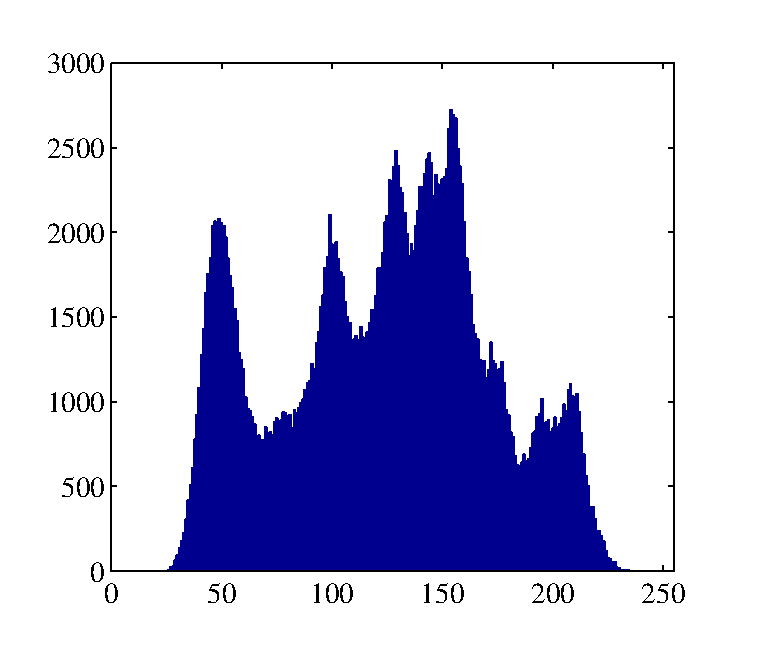
\includegraphics[width=0.4\textwidth]{figures/lena_hist.eps}
      \label{fig:lena_hist}}
    \subfigure[lena图像预测误差直方图]{
      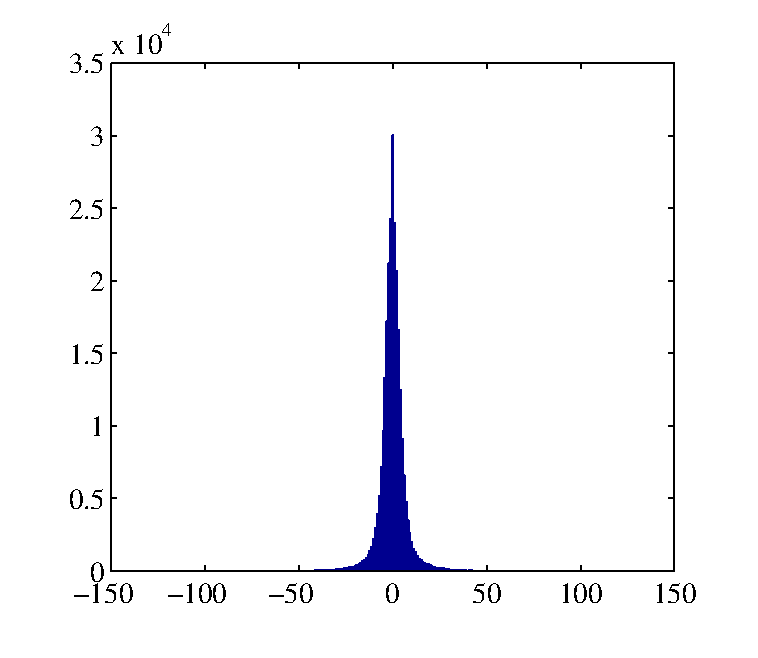
\includegraphics[width=0.4\textwidth]{figures/lena_diffhist.eps}
      \label{fig:lena_diffhist}}
    \caption{lena图像灰度直方图同预测误差直方图的比较}
    \label{fig:lena_hist_compare}
    \end{figure}
    由图中可以看出,同灰度直方图相比,预测误差直方图更加规则,呈Laplace分布,峰
    值位于0点,且比灰度直方图峰值更大。这就意味着使用预测误差直方图将得到更高的
    嵌入容量和更好的图像质量。从这个思路出发,大量的文献对该方法从预测方式到溢
    出问题进行了全面的改进。
  \vspace{-3.5mm}
  \item \textbf{差值扩展算法}
    \vspace{-2mm}
    \par
    这里我们将介绍Tian\cite{tian2003reversible}在2003年提出的差值扩展(Difference
    Expansion, DE)算法。在算法中,载体图像的像素被分为两两不相交的像素对,对每
    个像素对$(x_0, x_1)$,根据整数Haar变换,定义它们的整数均值和差值分别为
    $l=\lfloor (x_0-x_1)/2 \rfloor$和$h=x_1-x_0$。为了嵌入1比特消息$m \in \{0,
    1\}$,差值$h$被扩展为$h'=2h+m$。由整数Haar反变换,载密像素对$(y_0, y_1)$分别为
    $y_0=l-\lfloor h^*/2 \rfloor$和$y_1=l+\lfloor (h^*+1)/2 \rfloor$。通过简单地
    变形,我们得到:
    \begin{equation}
      \label{eq:de_marked_pair}
      \left\{ \begin{array}{l}
        y_0=2x_0-\lceil (x_0+x_1)/2 \rceil\\
        y_1=2x_1-\lceil (x_0+x_1)/2 \rceil+m
      \end{array} \right.
    \end{equation}
    这样,接收端可以通过提取$y_1-y_0$的最低比特位获得消息$m$,并通过$x_0=l^{'}-
    \lfloor h^{'}/2 \rfloor$和$x_1=l^{'}+\lceil h^{'}/2 \rceil$恢复原始像素对
    $(x_0, x_1)$,其中$l^{'}=\lfloor (y_0+y_1)/2 \rfloor$,$h^{'}=\lfloor (y_1-
    y_0)/2 \rfloor$。
    \par
    之后,Alattar\cite{alattar2003reversible,alattar2004reversible,
    alattar2004reversibleg}将差值扩展算法扩展到三像素对、四像素对及$n$像素
    对。在他的扩展中,$n$个像素被变换为一个均值$l$和一个有$n-1$个差值的向量
    $\boldsymbol{\vec{h}}$,对$\boldsymbol{\vec{h}}$的每个元素,都使用二像素对的
    方法进行扩展和消息嵌入。这样,嵌入率从二像素对的0.5 bpp提高到$(n-1)/n$ bpp。
    当选取的$n$合适时,嵌入容量和图像质量之间能得到很好地平衡。
    \par
    差值扩展技术作为可逆信息隐藏的一个基础技术,得到了充分地研究和发展,催生了大
    量新技术的诞生,如基于整数变换的嵌入方法,预测误差扩展算法等。在这些改进中,
    预测误差扩展算法得到了最为广泛的关注。同差值扩展利用两个像素的相关性不同,预
    测误差扩展用到了更大的邻域的相关性,因此可以预期,预测误差将会更加准确,因此
    算法性能将会更好。而预测误差扩展算法也因此成为了现在最为流行的可逆隐藏算法。
    下面将对预测误差扩展算法进行详细介绍。
  \vspace{-3.5mm}
  \item \textbf{预测误差扩展算法}
    \vspace{-2mm}
    \par
    首先先介绍一下预测误差扩展的一般流程:
    \begin{enumerate}[leftmargin=7em,label=\textbf{步骤 \arabic*:}]
      \item{对每个像素进行预测得到预测误差。首先对图像的每个像素$x_{i,j}$,使用一
        个预测器根据其邻域对其进行预测,得到预测值$x_{i,j}^{'}$。然后求预测误差
        $e_{i,j}=x_{i,j}-x_{i,j}^{'}$。}
      \item{通过计算每个预测误差的频数产生预测误差直方图,通常情况下预测误差服从
          Laplace分布,中心在0点或者0点附近。}
      \item{通过扩差和移位,对PEH进行修改。特别的,对预测误差$e_{i,j}$,它被扩展
        或移位为:
      \begin{equation}
        \label{eq:pee_embedding}
        e_{i,j}^{'}=\left\{ \begin{array}{ll}
          2e_{i,j}+m & if~~e_{i,j} \in [-T,T)\\
          e_{i,j}+T  & if~~e_{i,j} \in [T,+\infty)\\
          e_{i,j}-T  & if~~e_{i,j} \in (-\infty,-T)
        \end{array} \right.
      \end{equation}
      其中$T$是与嵌入容量有关的参数,$m$是消息比特。这里位于$[-T,T)$的预测误差被
      用来扩展以嵌入消息;位于$(-\infty,-T)\cup[T,+\infty)$的预测误差被向外移位,
      为扩展的差值提供空间,避免消息提取端的混淆。最后像素被修改为$e_{i,j}^{'}
      +x_{i,j}^{'}$。
      }
    \end{enumerate}
    \vspace{-2mm}
    \par
    由上面公式可以看出,嵌入容量取决于$T$,而像素失真的最大值也为$T$,所以载密图
    像的质量也与$T$有关,因此$T$的选取对算法有着重要的影响。
    \vspace{-2mm}
    \par
    在消息提取端,原始预测误差可以通过对载密图像的预测误差通过
    公式\ref{eq:pee_extraction}操作恢复。原始消息通过取位于$[-2T,2T)$区间内的预
    测误差$e_{i,j}^{'}$的最低比特位恢复。最终,原始图像通过已恢复的预测误差计算
    得出。
    \vspace{-5mm}
    \begin{equation}
      \label{eq:pee_extraction}
      e_{i,j}=\left\{ \begin{array}{ll}
        \lfloor e_{i,j}^{'}/2\rfloor & if~~e_{i,j}^{'} \in [-2T,2T)\\
        e_{i,j}^{'}-T  & if~~e_{i,j}^{'} \in [2T,+\infty)\\
        e_{i,j}^{'}+T  & if~~e_{i,j}^{'} \in (-\infty,-2T)
      \end{array} \right.
    \end{equation}
    \par
    通过利用预测误差直方图,预测误差扩展算法可以隐藏大量的消息信息,同时通过扩差
    和移位,图像失真得到了很好地控制。基于预测误差扩展的算法是当前可逆隐藏领域的
    研究热点和最有效的工具。最近提出的可逆隐藏算法大多数以预测误差扩展为框架,并
    对其中的部分环节进行改进。如使用更好的预测算法\cite{ou2013reversible},双层
    嵌入算法\cite{luo2010reversible},嵌入位置选择\cite{hong2012adaptive},二维
    直方图\cite{ou2013pairwise}等。
\end{itemize}

\subsection{基于整数变换的算法}
整数变换(Integer-to-Interger Transform)同样可以用于可逆隐藏算法中。正如前面所
看到的,差值扩展实质上也是一种整数变换算法。2007年,Coltuc和Chassery
\cite{coltuc2007very}提出了一种叫做可逆对比映射(Reversible Contrast Mapping)的
技术,应用了针对整数对的整数变换。这种算法不需要额外的可逆压缩算法,因此在计算复
杂度上有很高的效率。随后,该算法在2010年由Chen进行了改进\cite{chen2010reversible},
Chen将原始的可逆对比映射扩展到任意长度的整数序列。2010年,Wang
\cite{wang2010efficient}利用整数变换将差值扩展算法进行了推广。他们指出差值扩展算
法的嵌入规则可以被重组为一个整数对的变换,并将这种变换推广到了任意大小的像素块。
近期,通过从另一个视角审视差值扩展,Peng\cite{peng2012adaptive}提出了一种全新的
算法。算法首先根据预计算的失真将图像块分类,针对不同的图像块,使用不同的参数进行
整数变换。通过这种自适应的算法,消息更多地被隐藏在了平滑的图像块中,避免了嵌入噪
声块中造成的大失真,从而保证了较高嵌入容量下较好的图像质量。
\par
简而言之,基于整数变换的算法将两个或更多地像素组成一组,通过整数变换将消息分别嵌
入每一个组中,有较好的效果。但是,整数变换算法的预测算法并不准确,仅仅是使用一组
中像素的均值来预测该组中所有的像素。另外,同预测误差扩展算法相比,基于整数变换的
算法并不能控制图像的最大失真。由此可以确定,基于整数变换的算法仅仅对需要大嵌入容
量,而对图像质量有较少关注的应用中适用。

\subsection{排序技术}
在几乎所有的可逆隐藏算法中,都会使用位置地图(Location Map)来辅助消息提取端进行
消息提取和图像恢复。例如在差值扩展中,某些像素会出现上溢或下溢的问题,即当由于差
值的扩大而使得载密像素对不在$[0,255]$范围内时,这个像素对将不能用来隐藏消息。而为
了将这些像素对同那些载密像素对进行区分,就需要用一个位置地图对这些不能嵌入消息的
像素对进行记录:不能嵌入的像素对在位置地图中被设为1,可嵌入像素对被设为0。对于直
方图平移算法、预测误差扩展等算法都有相同的问题。通过对像素对或者像素进行打分、排
序,根据排序结果按顺序嵌入,最终的位置地图就可以被压缩到可以忽略不计的大小,因此
排序技术是可逆隐藏算法中一项非常重要的技术。
\par
使用排序技术的算法又被称为基于内容自适应的可逆隐藏算法(Content-Adaptive RDH),
最早的算法由Kamstra 和Heijmans 提出\cite{kamstra2005reversible}。文献对Tian的差
值扩展算法进行了改进,根据像素对的局部方差对像素对进行排序,依据排序结果依次对像
素对进行嵌入。注意到在差值扩展算法中,像素对的均值是不变的,只有其差值被修改,因
此像素对均值在嵌入端和提取端保持不变,双方都可以用此来计算局部方差。显然如果局部
方差越小,这个像素对应该在图像的纹理平滑区域,那么像素对的差值应越小,从而可嵌入
消息的可能性越大,位置地图越短。文献的实验结果表明使用排序的算法比原始算法有很大的
\begin{figure}[!h]
\centering 
\subfigure[排序前Airplane预测误差]{
  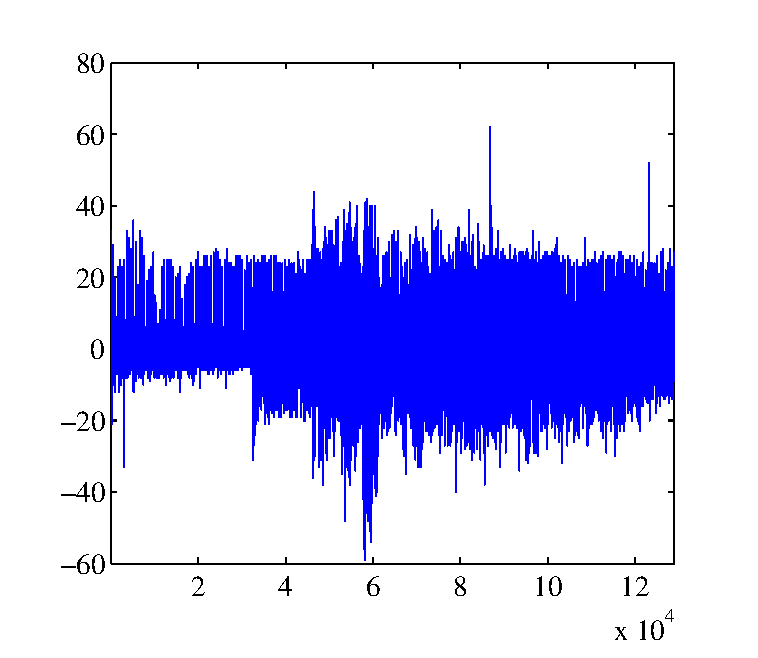
\includegraphics[width=0.4\textwidth]{figures/airplane_original_pe.eps}
  \label{fig:airplane_origin_pe}}
\subfigure[排序后Airplane预测误差]{
  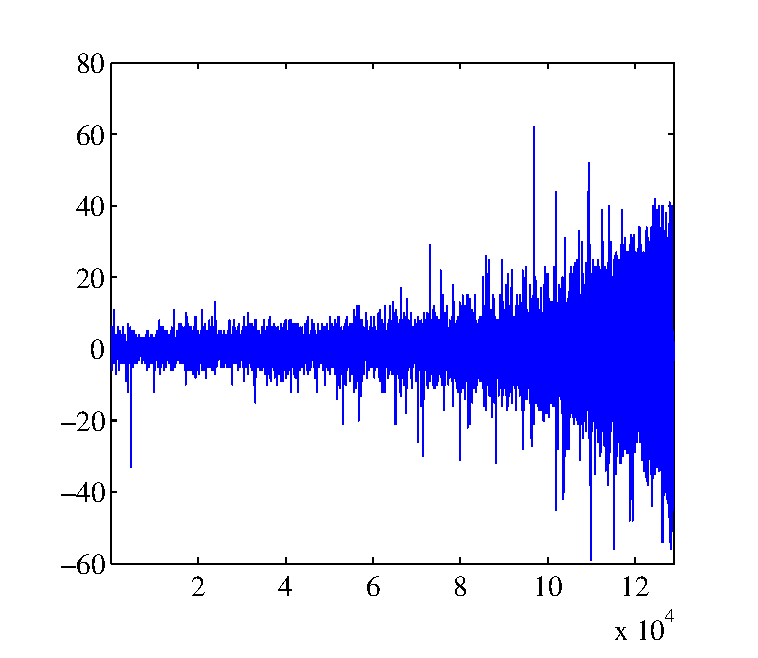
\includegraphics[width=0.4\textwidth]{figures/airplane_sorted_pe.eps}
  \label{fig:airplane_sorted_pe}}
\caption{lena图像灰度直方图同预测误差直方图的比较}
\label{fig:airplane_pe_compare}
\end{figure}
提升。最近的文献也表明\cite{sachnev2009reversible,hong2012adaptive},
将排序技术(或像素选择、嵌入位置选择等)同其他的可逆隐藏算法(如预测误差扩展)结
合,同样能使实验结果获得显著的提升。
\par
如图\ref{fig:airplane_pe_compare}所示,左侧是未排序之前Airplane图像的预测误差,
可以看到,预测误差在0附近波动很大。当利用邻域像素方差进行排序后得到的预测误差如
图\ref{fig:airplane_pe_compare}右侧所示,可以明显的看到,预测误差的绝对值呈现出
由小到大的增长顺序。由于小预测误差优先被用来嵌入,因此载密图像质量可以得到明显提
升。
\par
排序技术的关键是对每个像素或者像素对赋予一个关于图像复杂度的度量,以决定其位于图
像纹理平滑区域还是纹理复杂区域。然后,依据像素纹理复杂程度将纹理平滑的像素或像素
块排在靠前的位置。通过排序使得那些纹理相对平滑的区域被用来嵌入的可能性变大。而由
于纹理越平滑,预测误差就越小,从而用来嵌入时失真也越小。由此可见,排序技术对于改
善可逆信息隐藏的效果有着至关重要的作用。



\section{彩色图像可逆隐藏算法}
基于灰度图像的可逆隐藏算法得到了信息隐藏领域的广泛和深入的研究。但是在现实生活中
,使用最多的还是彩色图像而非灰度图像。但是针对彩色图像的可逆隐藏算法却没有得到深
入的研究。在2013年,Li等人提出了一种基于彩色图像通道相关性的可逆隐藏算法
\cite{li2013reversible}。文献中发现了这样一种彩色图像的通道相关性:一个通道
内的图像边缘方向同另外通道内的图像边缘方向是相同的。图\ref{fig:lena_canny}给出了
Lena图像RGB三个通道Canny算子求得的边缘:
\begin{figure}[!hbt]
\centering 
\subfigure[Canny边缘-R通道]{
  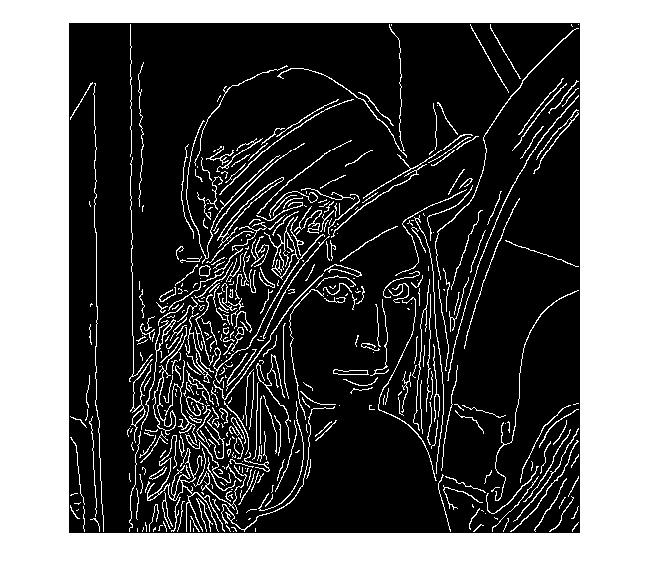
\includegraphics[width=0.3\textwidth]{figures/lena_r_canny.jpg}
  \label{fig:lena_r_canny}}
\subfigure[Canny边缘-G通道]{
  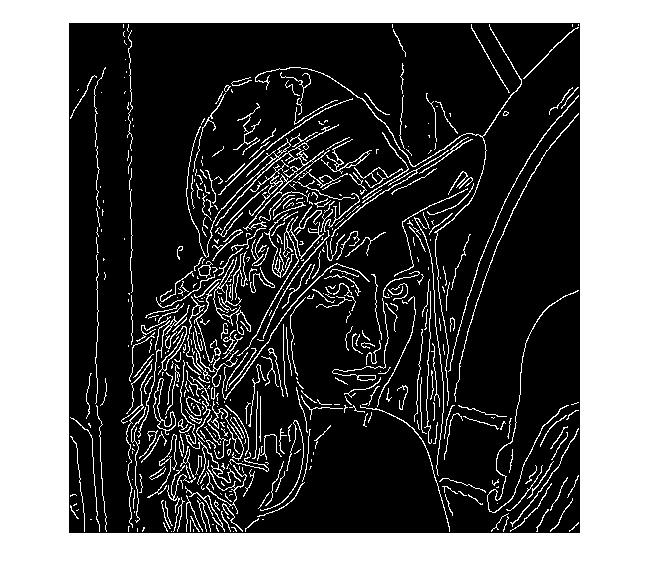
\includegraphics[width=0.3\textwidth]{figures/lena_g_canny.jpg}
  \label{fig:lena_g_canny}}
\subfigure[Canny边缘-B通道]{
  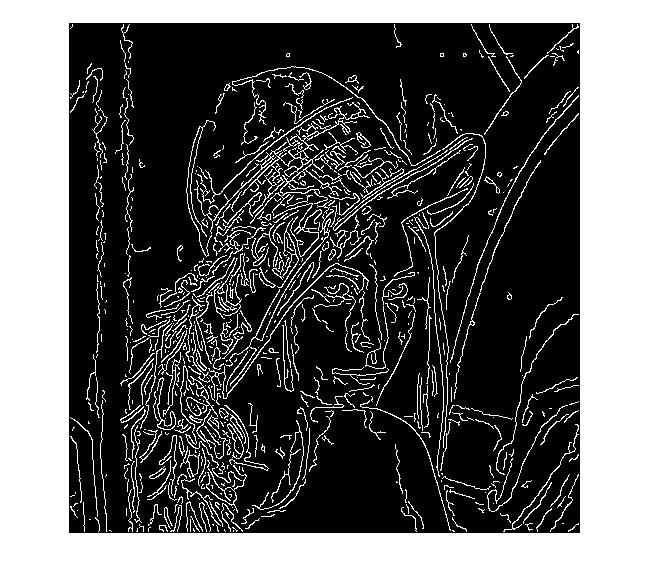
\includegraphics[width=0.3\textwidth]{figures/lena_b_canny.jpg}
  \label{fig:lena_b_canny}}
\caption{Lena图像三个通道边缘信息}
\label{fig:lena_canny}
\end{figure}
从图像中可以看出,在一个通道内的边缘部分,在另一个通道内也基本是边缘部分,同时边
缘方向也基本相同。基于此,文中的预测算法能够较好地对纹理复杂区域的像素进行较好的
预测。
\begin{figure}
  \centering
  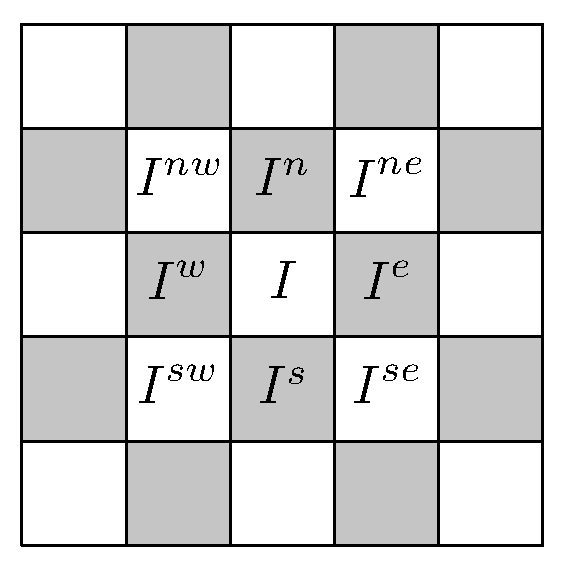
\includegraphics[width=0.3\textwidth]{figures/pixel_neighbourhood.eps}
  \caption{像素$I$的邻域像素}
  \label{fig:pixel_neighbour}
\end{figure}
\par
算法的预测过程如下:设当前通道内的像素为$I_c$,对应的参考通道内的像素为$I_r$。为
了决定当前像素是否在边缘区域,定义两个值。一个表示$I_r$与其邻域内8个像素的距离,
设为$D_m$,像素的8个邻域如图\ref{fig:pixel_neighbour}所示。
\begin{equation}
  D_m=\left|\sum_{k=1}^{8}\lambda_{m}^{k}I_{r}^{k}-I_r\right|
\end{equation}
其中$\lambda_{m}^{k}=1/8$,$I_{m}^{k}(k=1,2,\cdots,8)$表示如图\ref{fig:pixel_neighbour}
所示的8个邻域点。显然当一个像素位于纹理平滑区域时,$D_m$会很小。
\par
另一个值与边缘有关。通过对一个系数向量$\boldsymbol{\lambda_e}$取不同的取值,得到
另一个值$D_e$:
\begin{equation}
  D_e=\left|\sum_{k=1}^{8}\lambda_{e}^{k}I_{r}^{k}-I_r\right|
\end{equation}
$D_e$可以从多个方向的预测误差中选出。文献中使用了四个预测误差:
\begin{equation}
  \begin{array}{ll}
  D_h=\left|\frac{\displaystyle I_r^{w}+I_r^{e}}{\displaystyle 2}-I_r\right| &
  D_v=\left|\frac{\displaystyle I_r^{n}+I_r^{s}}{\displaystyle 2}-I_r\right|\\
  D_d=\left|\frac{\displaystyle I_r^{nw}+I_r^{se}}{\displaystyle 2}-I_r\right| &
  D_{ad}=\left|\frac{\displaystyle I_r^{ne}+I_r^{sw}}{\displaystyle 2}-I_r\right|\\
  \end{array}
\end{equation}
则$D_e=min\{D_h,D_v,D_d,D_{ad}\}$,$\boldsymbol{\lambda_e}$取相应的取值,例如当
$D_e=D_h$时,$\boldsymbol{\lambda_e}=(0,0,0,1/2,1/2,0,0,0)$。
\par
我们知道,在图像的纹理平滑区域,一个像素同它邻域像素的值相似,因此,$D_m$和$D_e$
都应接近于0,它们的差也接近0;另一方面,在图像的纹理复杂区域,一个像素同它边缘方
向上的各个像素相似,而与其他邻域的像素有较大差异,因此$D_m$较大,而$D_e$接近于0,
从而它们的差值也较大。因此,设定临界值$\tau$,当$|D_m-D_e|>\tau$,像素位于纹理复
杂区域,$|D_m-D_e|\le\tau$时,图像位于纹理平滑区域。从而当前通道内的预测值为:
\begin{equation}
  \hat{I}_c=\left\{ \begin{array}{ll}
    \frac{\displaystyle I_c^w+I_c^e+I_c^n+I_c^s}{\displaystyle 4} &
    |D_m-D_e|\le\tau\\
    \sum_{k=1}^{8}\lambda_e^kI_c^k &
    |D_m-D_e|>\tau
  \end{array} \right.
\end{equation}
基于此预测值,获得预测误差直方图,利用预测误差扩展和排序技术,进行可逆隐藏。经试
验分析,该算法同简单地将灰度图像的可逆隐藏算法分别应用到三个通道相比,能得到更高
的嵌入容量,更好的图像质量。
\par
本论文的算法将对该算法进行一定地改进,具体内容将在下一章给出。

  \chapter{基于通道相关性的彩色图像可逆隐藏}
\label{c:proposed}
在本章中将首先对本论文提出的二阶预测算法和嵌入算法进行介绍,然后将给出新的像素排
序算法,在第三节会给出完整的嵌入流程,最后是对实验结果的分析总结。


\section{预测嵌入}
尽管一个像素的三个通道之间存在一定的联系,但是它们并没有明显的通道相关性。下图是
lena图像红-绿通道像素差的直方图同预测误差直方图的对
\begin{figure}[!h]
\centering 
\subfigure[lena图像R-B直方图]{
  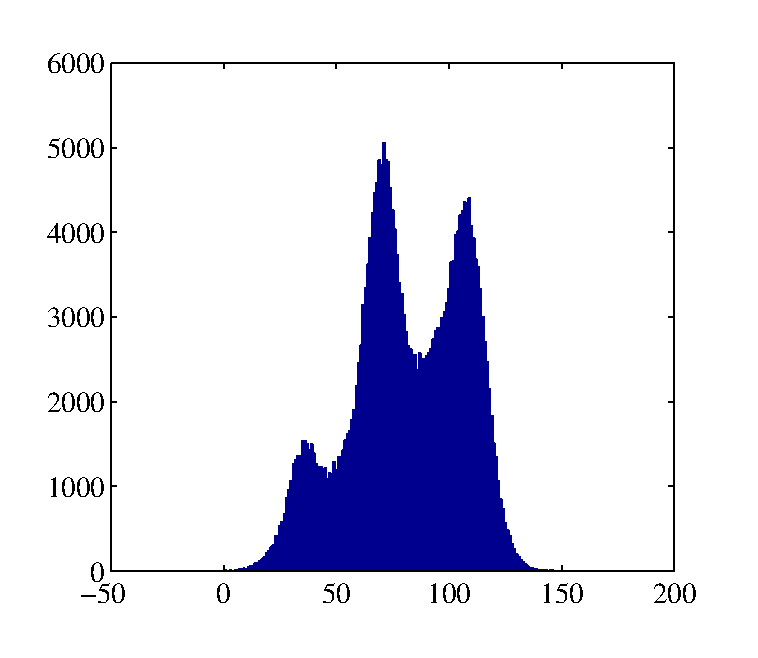
\includegraphics[width=0.4\textwidth]{figures/lena_r_g.eps}
  \label{fig:lena_rg_hist}}
\subfigure[lena图像预测误差直方图]{
  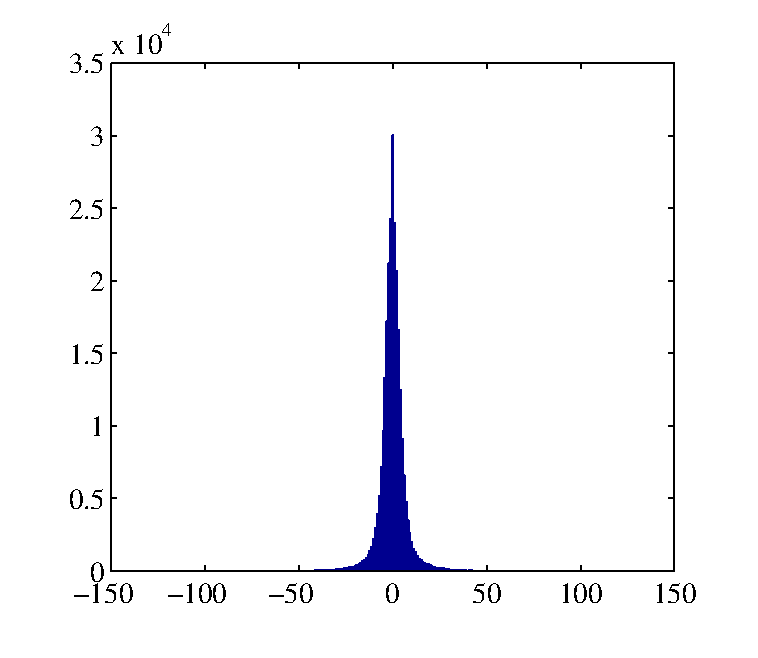
\includegraphics[width=0.4\textwidth]{figures/lena_diffhist.eps}
  \label{fig:lena_diffhist2}}
\caption{lena图像灰度直方图同预测误差直方图的比较}
\label{fig:lena_rg_pe_compare}
\end{figure}
比。我们可以看到直接的像素差的方差很大,且没有明显的规律可寻。因此,现在常用的
算法都针对预测误差进行平移扩展。
\par
然而,一般的预测算法在图像的纹理复杂区域的预测效果却并不理想。在这种情况下,由于
邻域像素同被预测像素的巨大差异,预测值通常与正确值有着很大的差异。另一方面,由于
彩色图像存在三个通道,通道间的高度的相关性为在图像纹理复杂区域的预测提供了帮助,
当对一个通道内的像素进行预测时,我们可以利用另一个通道的信息来辅助当前通道进行更
准确的预测。图\ref{fig:lena_rgb_pe_compare}分别是Lena图像利用一般的预测算法分别
对RGB三个通道进行预测之后的预测误差图。
\begin{figure}[!h]
\centering 
\subfigure[R通道预测误差图]{
  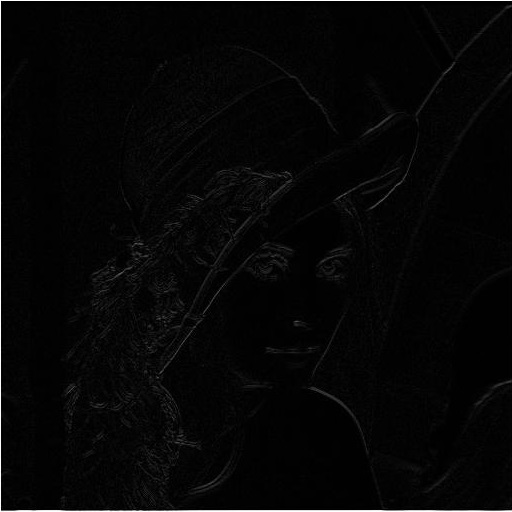
\includegraphics[width=0.3\textwidth]{figures/lena_pe_r.jpg}
  \label{fig:lena_rpe_hist}}
\subfigure[G通道预测误差图]{
  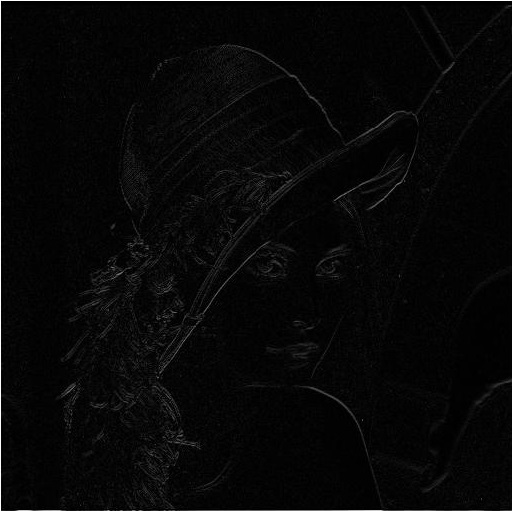
\includegraphics[width=0.3\textwidth]{figures/lena_pe_g.jpg}
  \label{fig:lena_gpe_hist}}
\subfigure[B通道预测误差图]{
  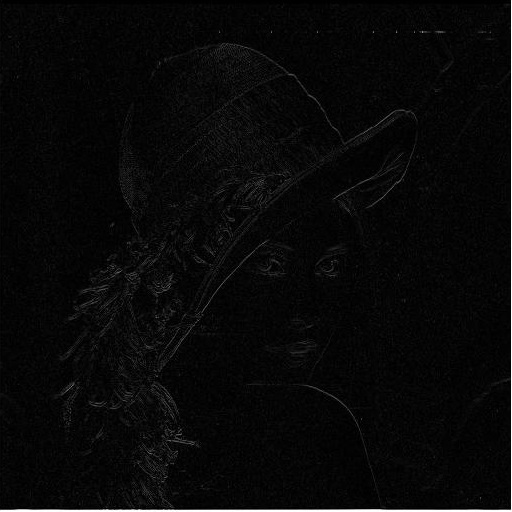
\includegraphics[width=0.3\textwidth]{figures/lena_pe_b.jpg}
  \label{fig:lena_bpe_hist}}
\caption{lena图像三个通道预测误差图像对比}
\label{fig:lena_rgb_pe_compare}
\end{figure}
从图中我们可以看到,如果一个像素在当前通道内可以被准确预测,那么在另外两个通道
也基本可以被准确预测;对于纹理复杂区域,在三个通道基本都不能做出很准确的预测,
然而三个通道的预测误差却很相似。因此,如果我们在一个通道内对一个像素求出了一个
预测误差$e$,那么我们可以推测在另一个通道内的预测误差应该同$e$是很接近的。
\par
这样,在本文提出的可逆隐藏算法中,数据同样是分别嵌入到每一个通道中。但是在对当
前的通道进行预测的过程中,我们会选取另外一个参考通道同样进行一次预测,得到一个
参考预测误差对当前通道的预测误差进行二次预测。在本文的算法中,依然使用Sachev提
出的棋盘格格式的两轮预测的算法。对于一个像素$I$,设当前通道内的像素表示为$I_c$,
参考通道内的像素表示为$I_r$。图\ref{fig:pixel_neighbour2}表示一个像素的8个邻域
像素。
\begin{figure}
  \centering
  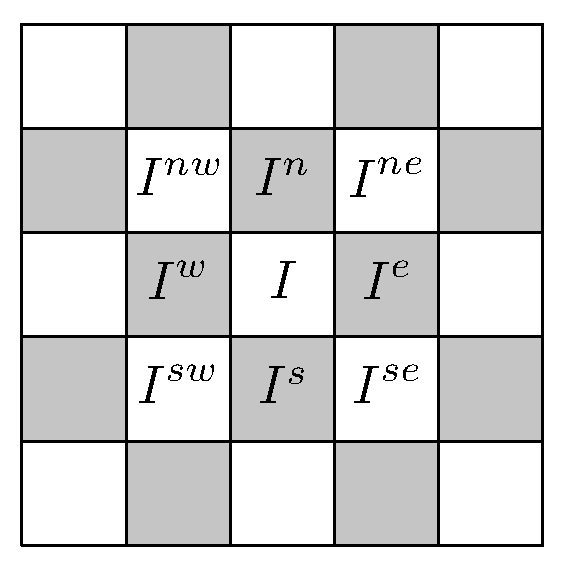
\includegraphics[width=0.3\textwidth]{figures/pixel_neighbourhood.eps}
  \caption{像素$I$的邻域像素}
  \label{fig:pixel_neighbour2}
\end{figure}
\par
首先对当前通道内的像素$I_c$求其预测值$\hat{I}_c$和通道内一阶预测误差$e_{1c}$:
\begin{eqnarray}
  & \displaystyle \hat{I}_c=
    \left\lfloor \sum_{k=1}^8\lambda_c^kI_c^k+0.5 \right\rfloor & \\
  & e_{1c}=I_c-\hat{I}_c &
  \label{eq:current_predict}
\end{eqnarray}
\par
其中$\lambda_c^k$为预测算法中对邻域像素的权重,可以如文献
\cite{sachnev2009reversible}中,选取上下左右权重为$1/4$,或者如文献
\cite{luo2010reversible}中,基于插值自适应的选取系数,或者如文献
\cite{li2013reversible}中的权重选取算法;$I_c^k$为像素的8个邻域点。显然,在纹理
平滑区域,$e_{1c}$的值应该较小,而在纹理平滑区域,$e_{1c}$的值较大。这样,对参
考通道的像素求其预测值$I_r$和通道内一阶预测误差$e_{1r}$:
\begin{eqnarray}
  & \displaystyle \hat{I}_r=
    \left\lfloor \sum_{k=1}^8\lambda_r^kI_r^k+0.5 \right\rfloor & \\
  & e_{1r}=I_r-\hat{I}_r &
  \label{eq:reference_predict}
\end{eqnarray}
\par
此时我们得到了当前通道预测误差$e_{1c}$和参考通道预测误差$e_{1c}$,我们求当前像素
$I_c$的二阶预测误差$e_2$:
\begin{equation}
  e_2=e_{1c}-e_{1r}
  \label{eq:second_predict}
\end{equation}
\par
我们知道,在平滑区域预测算法都可以预测的很准确。这样$e_{1c}$和$e_{1r}$都接近于0,
二阶误差$e_2$同样接近于0;而对于纹理复杂区域,$e_{1c}$和$e_{1r}$都相对较大,但
是由于前面所述的通道间相关性,二阶误差$e_2$同样会较小。
\par
预测算法的效果的好坏通常由预测误差直方图的陡峭程度来衡量,数值化之后就是预测误差
的熵值。熵越小,预测结果就越准确。我们对UCID数据库\cite{schaefer2003ucid}中超
1300副图像都进行了考察。对每一幅图像,我们计算了论文预测算法的熵值和另外几种算法
的熵值。从图\ref{fig:entropy_compare}中可以看出,几乎对所有的图像我们提出的预测
算法的熵值都比以往算法的熵值要小。这在统计上证明了提出的预测算法可以比以往算法
获得更准确的预测误差。
\par
接下来,参考传统的预测误差扩展算法,定义两个阈值$T_r$和$T_l$,将预测误差直方图
分为一个扩展区域和两个平移区域。对不同区域的二阶预测误差$e_2$进行扩展或者平移,
即:
\begin{equation}
  e_2^{'}=\left\{ \begin{array}{ll}
    2e_2+b & if~~e_2 \in [T_r,T_l)\\
    e_2+T_r & if~~e_2 \ge T_r\\
    e_2+T_l & if~~e_2<T_l
  \end{array} \right.
  \label{eq:second_pe_embedding}
\end{equation}
\begin{figure}
  \centering
  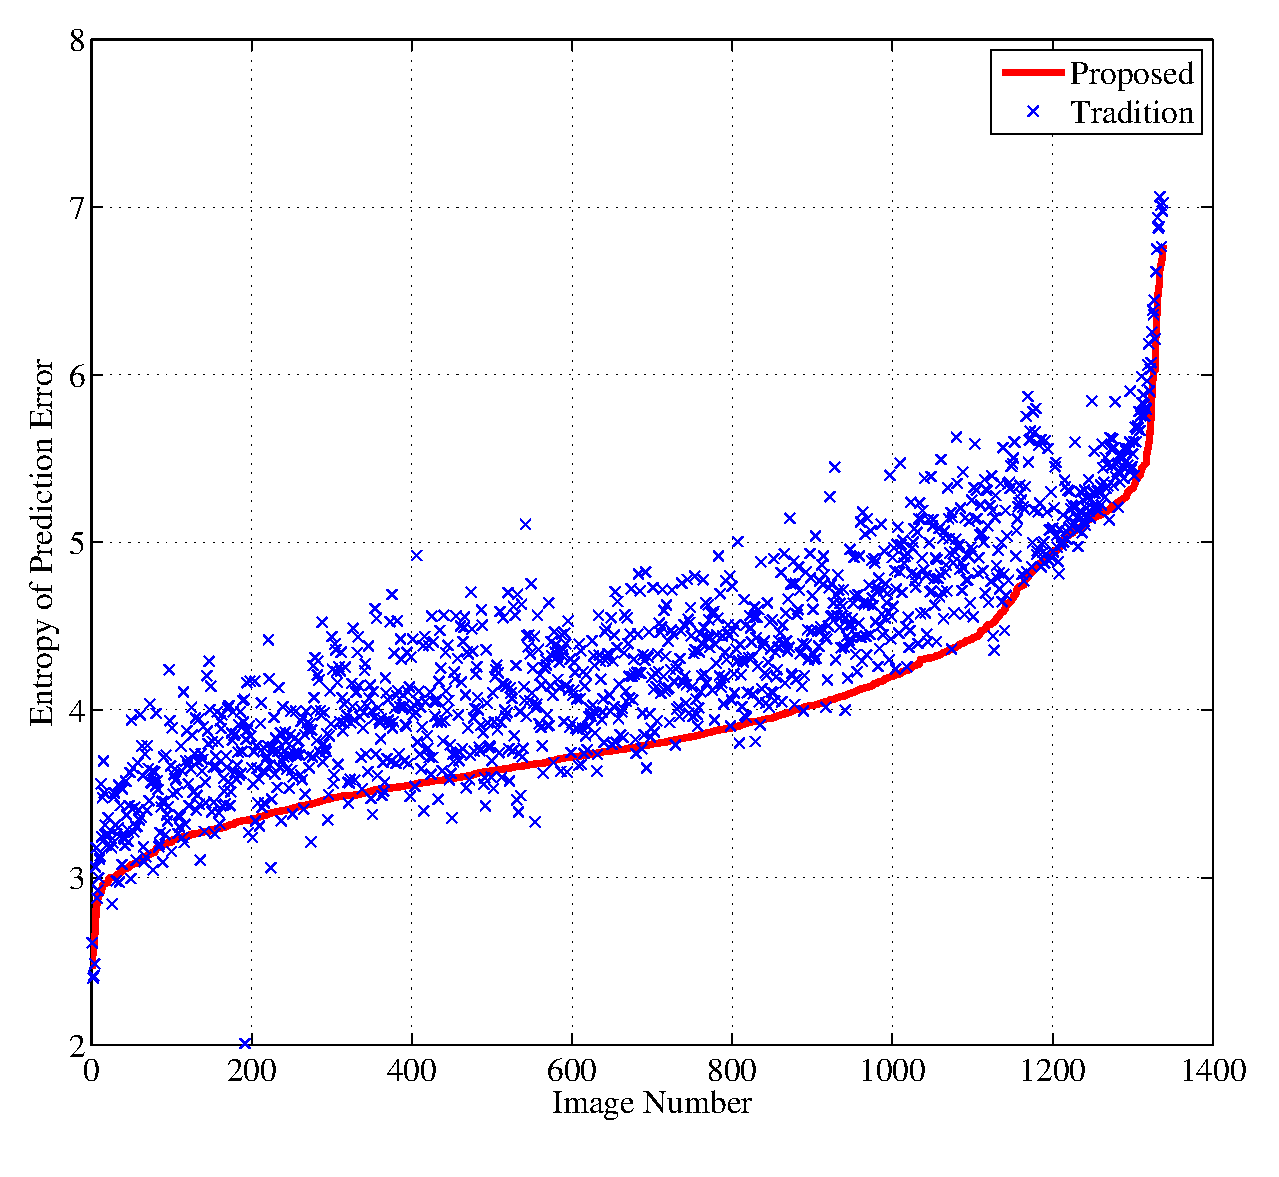
\includegraphics[width=0.65\textwidth]{figures/entropy_compare.eps}
  \caption{预测误差直方图熵比较}
  \label{fig:entropy_compare}
\end{figure}
其中$b\in\{0,1\}$为1比特要嵌入的信息。将修改后的二阶误差加到使用参考通道预测的
一阶预测误差上得到:
\begin{equation}
  e_{1c}^{'}=e_{1r}+e_2^{'}
  \label{eq:cur_first_pe_embedding}
\end{equation}
最后将修改后的一阶误差加到当前通道的预测值上得到修改后的像素值:
\begin{equation}
  I_c^{'}=\hat{I}_c+e_{1c}^{'}
  \label{eq:marked_pixel}
\end{equation}
\par
在消息提取端,首先求当前通道的预测值$\hat{I}_c$和参考通道的预测值$\hat{I}_r$,
求得修改后的当前通道的误差$e_{1c}^{'}$和参考误差$e_{1r}$,从而计算得出修改后的
二阶误差$e_2^{'}$。显然消息比特$b$为二阶误差的最低有效位,即:
\begin{equation}
  \begin{array}{ll}
    \displaystyle b=e_2^{'}-2\left\lfloor\frac{e_2^{'}}{2}\right\rfloor & 
    if~~e_2^{'}\in[2T_l,2T_r)
  \end{array}
  \label{eq:data_extraction}
\end{equation}
\par
为了恢复原始像素,首先恢复原始二阶预测误差:
\begin{equation}
  e_2=\left\{ \begin{array}{ll}
    \displaystyle \left\lfloor\frac{e_2^{'}}{2}\right\rfloor &
    if~~e_2^{'} \in [2T_r,2T_l)\\
    e_2^{'}-T_r & if~~e_2^{'} \ge 2T_r\\
    e_2^{'}-T_l & if~~e_2^{'}<2T_l
  \end{array} \right.
  \label{eq:second_pe_restoration}
\end{equation}
从而根据\ref{eq:second_predict}和\ref{eq:current_predict}的逆过程恢复当前通道
的一阶预测误差和原始像素。




\section{像素排序与位置地图}
嵌入算法的效果可以通过进一步的排序得到提升。根据像素的纹理复杂度将像素进行排序,
使纹理平滑的像素,即预测误差更小的像素尽可能多的被修改。根据嵌入公式,我们知道,
被嵌入的像素的失真为其预测误差,被移动的像素失真为阈值$T_r$或者$T_l$。由此可以
知道,当修改的像素大多数时候是小误差的像素时,图像失真就会较小。在本节中,将给
出对像素排序和位置地图的细节和数学推导。
\par
如前文所述,理想化的图像预测误差是服从标准拉普拉斯分布的。为了细致的研究预测误
差的分布特征,以在排序中对其加以利用,我们将独立的对每一个像素点的预测误差分布
进行研究。以某个像素点为例,其邻域像素如图\ref{fig:pixel_neighbour2}所示。
\par
首先对当前像素$I$,取其$3\times3$邻域的上下左右四个邻域像素,求得四个差值:
\begin{eqnarray}                           
  & d_1=I^w-I^n & \\
  & d_2=I^n-I^e & \\
  & d_3=I^e-I^s & \\
  & d_4=I^s-I^w &
\end{eqnarray}
设预测误差$e_1$服从参数为$(\mu_1,\lambda_1)$的拉普拉斯分布,令:
\begin{equation}
  \mu_1^1=\frac{1}{2}(d_1+d_3), \mu_1^2=\frac{1}{2}(d_2+d_4)
\end{equation}
取$\mu_1^1$,$\mu_1^2$中较小的一个作为该预测误差分布的期望$\mu_1$再令:
\begin{equation}
  \lambda_1=\sqrt{\frac{1}{4\times2}\sum_{k=1}^{4}(d_k-\mu_1)^2}
\end{equation}
作为该点拉普拉斯分布的参数$\lambda_1$,(标准拉普拉斯分布中方差为$2\lambda_1^2$),
我们就可以得到该待嵌入像素点的一个分布的估计:
\begin{equation}
  f(x)=\frac{1}{2\lambda_1}e^{-\frac{|x-\mu_1|}{\lambda_1}}
  \label{eq:laplace_distr}
\end{equation}
其概率密度函数图像如图\ref{fig:laplace_distr}:
\begin{figure}[!h]
\centering 
\subfigure[概率分布情况1]{
  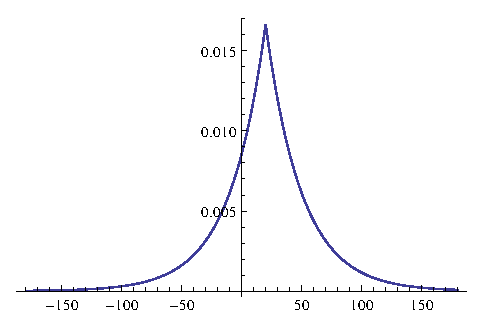
\includegraphics[width=0.3\textwidth]{figures/laplace1.eps}
  \label{fig:laplace1}}
\subfigure[概率分布情况2]{
  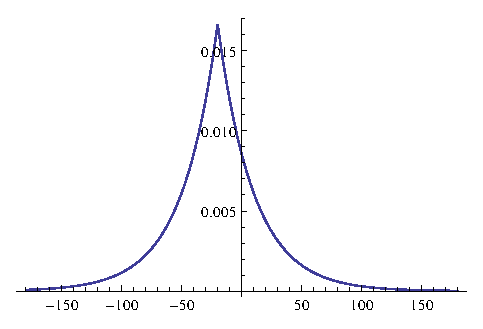
\includegraphics[width=0.3\textwidth]{figures/laplace2.eps}
  \label{fig:laplace2}}
\subfigure[$g(x)$概率分布图]{
  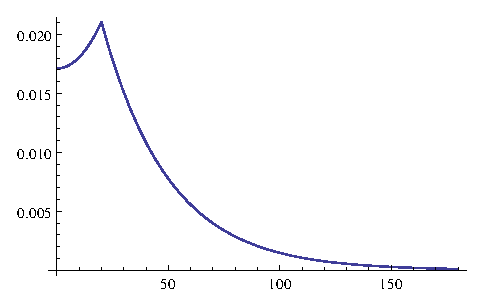
\includegraphics[width=0.3\textwidth]{figures/laplace3.eps}
  \label{fig:laplace_distr_new}}
\caption{$f(x)$和$g(x)$概率分布图}
\label{fig:laplace_distr}
\end{figure}
\par
由图像可以看出,$\mu$到$y$轴的距离大小可以用来反映预测误差的准确程度,$\mu$到$y$
轴越近,则预测误差越接近0,因而预测的越准确。
\par
由于使用了$\mu$到$y$轴的距离来衡量预测误差的准确程度,因此可以将拉普拉斯分布位于
$x$轴负半边的图像取绝对值,翻转到$x$轴正半边,得到一个新的概率密度图像如图\ref{fig:laplace_distr_new}:
\par
设其概率密度函数为$g(x)$,其期望值是一个与$\mu$的绝对值(即$\mu$到0轴的距离)正
相关的数(具体计算结果将在下文给出),因此我们可以利用$g(x)$的期望值$E[g(x)]$作
为当前像素预测误差准确性的度量,用其对像素进行排序,这是本文排序算法的核心。
\par
设当前待嵌入像素的预测误差的分布为公式\ref{eq:laplace_distr},不妨假设此时$\mu>0$
(小于0时对 取绝对值即可),则此时$g(x)$是一个分段函数:
\begin{equation}
  g(x)=\left\{ \begin{array}{ll}
    \frac{1}{2\lambda}e^{-\frac{\mu-x}{\lambda}}+\frac{1}{2\lambda}e^{-\frac{\mu+x}{\lambda}} &
    if~~0\le x\le\mu\\
    \frac{1}{2\lambda}e^{-\frac{x-\mu}{\lambda}}+\frac{1}{2\lambda}e^{-\frac{\mu+x}{\lambda}} &
    if~~x\ge\mu\\
  \end{array} \right.
  \label{eq:second_pe_embedding}
\end{equation}
其期望为:
\begin{equation}
  E[g(x)]=\int_0^{\infty}xg(x)dx=\lambda e^{-\frac{\mu}{\lambda}}+\mu
\end{equation}
则对当前像素预测误差准确程度的度量为$\lambda e^{-\mu/\lambda}+\mu$。其中$\mu$和
$\lambda$由前文可知。可以很容易的看出,$E$是关于$\mu$和$\lambda$的递增函数,显然
$\mu$和$\lambda$越小,相应地$E$也越小,从而表示预测越精准。因此$E$能很好地反映出
当前像素邻域的纹理复杂性和预测精准度。
\par
在本算法中,由于使用了参考通道的预测误差去预测当前通道的预测误差,因此仅仅使用$E$
来进行排序是不够的。我们在算法中使用
\begin{equation}
  E^{'}=|E_c-E_t|
  \label{eq:sorting_param}
\end{equation}
的方式,表示当前像素两个通道的纹理复杂度的差,差值越小,则表示两个通道在这个像
素点处的结构越相似,因此二阶预测误差也更准。
\par
然而,即使是完美的排序算法也无法避免像素的上溢和下溢问题,因此需要引入位置地图。
我们使用的位置地图构建算法同文献\cite{li2013reversible}的基本相同。当当前像素不
能通过公式\ref{eq:second_pe_embedding}被修改两次时,将在位置地图上记录该像素。
如果像素可以被修改一次,则在位置地图中表示为0;如果像素不能被修改,则在位置地图
中表示为1。然而,由于在预测过程中,使用的邻域像素有可能是载密像素,那么要记录在
位置地图中的像素只有在嵌入的过程中才能确定。即位置地图的构建要在消息嵌入的过程
中同步进行。而如果位置地图和一些辅助信息仍然按照消息的嵌入方式进行嵌入,则有可
能造成新的像素发生上溢或下溢,从而可能要构造另一个位置地图,这样嵌入过程有可能
一直进行。为了解决这个问题,我们将位置地图等信息嵌入到那些值用上、下、左、右四
个邻域进行预测的像素中。这样,嵌入位置地图的那些像素可以提前判断是否会发生上下
溢,从而避免了位置地图的多次构建。



\section{完整流程}
\begin{itemize}
  \setlength{\parindent}{2em}
  \vspace{-2mm}
  \item \textbf{嵌入过程}
    \vspace{-2mm}
    \par
    在本节,基于我们提出的预测算法和排序算法,我们将给出详细的嵌入算法流程。同文
    献\cite{li2013reversible}相同,参考图\ref{fig:three_channel_embedding},我们
    首先以绿色通道为参考通道,将消息嵌入到红色和绿色通道。当嵌入到绿色通道时,以
    已嵌入的红色通道为参考通道。同时,在一个通道中,所有的像素被分为两个集合,以
    灰色和白色像素表示。消息将分为两个阶段分别嵌入到两个集合中,在第一个阶段,将
    消息嵌入到白色的像素中,步骤如下:
    \vspace{2mm}
    \begin{algorithm}[!h]
      \floatname{algorithm}{算法}
      \renewcommand{\algorithmicrequire}{\textbf{输入:}}
      \renewcommand\algorithmicensure {\textbf{输出:}}
      \caption{嵌入算法步骤}
      \label{alg:embedding_step} 
      \begin{algorithmic}[1]
        \REQUIRE ~~\\ %算法的输入参数:Input
        当前通道像素序列,参考通道像素序列,嵌入容量,嵌入消息
        \ENSURE ~~\\ %算法的输出:Output
        载密像素序列
        \vspace{2mm}
        \STATE 设当前阶段待嵌入像素为$\boldsymbol{I}=\{I_1,\dots,I_n\}$,对每
        个像素$I_i$,按照公式\ref{eq:sorting_param}计算其排序权重值$\boldsymbol{V}
        =\{V_1,\dots,V_n\}$,依照$\boldsymbol{V}$的升序,对$\boldsymbol{I}$进行
        排序,得到排序后的像素$\boldsymbol{\tilde{I}}=\{\tilde{I}_1,\dots,
        \tilde{I}_n\}$。
        \STATE 设定阈值初值$T_l$和$T_r$。
        \STATE 将消息嵌入到排序后的像素$\boldsymbol{\tilde{I}}$。对每一个像素
        $\tilde{I}_i (i=1,2,\dots)$,首先根据
        公式\ref{eq:current_predict}--\ref{eq:second_predict}计
        算其预测值和预测误差。根据公式\ref{eq:second_pe_embedding}将消息嵌入到
        像素$\tilde{I}_i$中,得到嵌入消息的像素$\tilde{I}_i^{'}$。然后构建位置地
        图$LM$。如果$\tilde{I}_i^{'}\notin [0,255]$,则$LM(j)=1$,$j=j+1$,将
        $\tilde{I}_i^{'}$改回$\tilde{I}_i$;如果$\tilde{I}_i^{'}\in [0,255]$,但
        是再次嵌入消息后结果不属于$[0,255]$,则$LM(j)=0$,$j=j+1$。
        \STATE 当消息嵌入完成后,记录最后一个嵌入的像素位置为$e$。则
        对$\tilde{I}_i (i=e+1, e+2,\dots, n)$,按照嵌入算法检测所有可嵌入
        的像素的个数,同时记录相应地位置地图。如果可嵌入的像素个数不足以嵌入压缩
        后的$LM$和另外40比特,则将$T_l$减小1(或者将$T_r$增加1),重新开始步骤4。
        否则将$LM$进行可逆压缩,记录压缩后的长度为$l$。
        \STATE 记录当前前40个像素的最低有效位(LSB)为$S_{LSB}$,然后将它们替换为
        $T_r$(8比特),$T_l$(8比特),$l$(8比特)和$e$(16比特)的二进制表示。
        最后将$S_{LSB}$和压缩后的$LM$按照公式\ref{eq:second_pe_embedding}嵌入到
        $e$位置之后的像素中。
      \end{algorithmic}
    \end{algorithm}
    \vspace{-6mm}
    \par
    第二阶段同第一阶段基本相同,只是将待嵌入的像素换成被标记成灰色的像素。
  \vspace{-3.5mm}
  \item \textbf{提取过程}
    \vspace{-2mm}
    \par
    同嵌入过程相反,我们依次从绿色、蓝色、红色通道提取消息,一个通道内的消息提
    取过程也于嵌入过程相反。对每个通道,首先对灰色像素进行提取,提取过程主要分
    为四步。
    \begin{algorithm}[!h]
      \floatname{algorithm}{算法}
      \renewcommand{\algorithmicrequire}{\textbf{输入:}}
      \renewcommand\algorithmicensure {\textbf{输出:}}
      \caption{提取算法步骤}
      \label{alg:embedding_step} 
      \begin{algorithmic}[1]
        \REQUIRE ~~\\ %算法的输入参数:Input
        当前通道载密像素序列,参考通道像素序列
        \ENSURE ~~\\ %算法的输出:Output
        当前通道原始像素,消息
        \vspace{2mm}
        \STATE 找到所有要提取的像素$\boldsymbol{I^{'}}=\{I_1^{'},\dots,I_n^{'}\}$,
        对每个像素进行平滑度打分,得到$\boldsymbol{V}=\{V_1,\dots,V_n\}$,依照
        $\boldsymbol{V}$的升序对载密像素进行排序得到$\boldsymbol{\tilde{I}^{'}}=
        \{\tilde{I}_1^{'},\dots,\tilde{I}_n^{'}\}$
        \STATE 从前40个载密像素提取LSB位,分别恢复$T_r$,$T_l$,$l$和$e$。
        \STATE 按照相反的顺序,从$\{\tilde{I}_{e+l+40}^{'},\dots,\tilde{I}_e^{'}\}$
        的LSB位提取$S_{LSB}$和压缩的$LM$,同时恢复原始的$\{I_{e+l+40},\dots,
        I_{e+1}\}$,对$LM$解压缩,得到原始的位置地图$LM$。
        \STATE 替换前40个载密像素的LSB位为$S_{LSB}$,恢复前40个像素。通过公式%
        \ref{eq:data_extraction}和\ref{eq:second_pe_restoration}提取像素中嵌入
        的消息并恢复原始像素值。
      \end{algorithmic}
    \end{algorithm}
    \vspace{-6mm}
    \par
    第二阶段同第一阶段基本相同,只是将载密像素换成被标记为白色的像素。
    \begin{figure}[!h]
      \centering 
      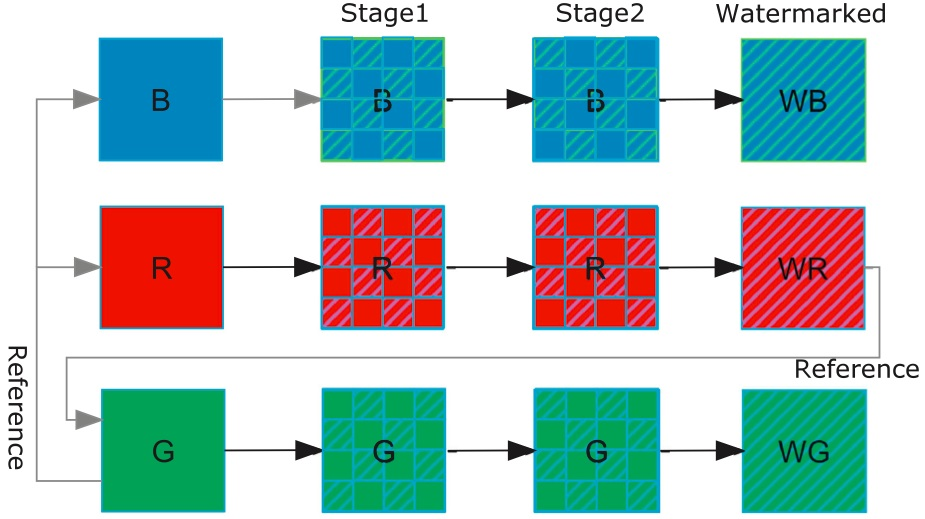
\includegraphics[width=0.65\textwidth]{figures/three_channel_embedding.jpg}
      \caption{彩色图像三个通道嵌入流程图}
      \label{fig:three_channel_embedding}
    \end{figure}
\end{itemize}



\section{实验结果}
\par
在本节,我们将给出所提出的可逆隐藏算法的实验结果。
\begin{figure}[!h]
  \centering 
  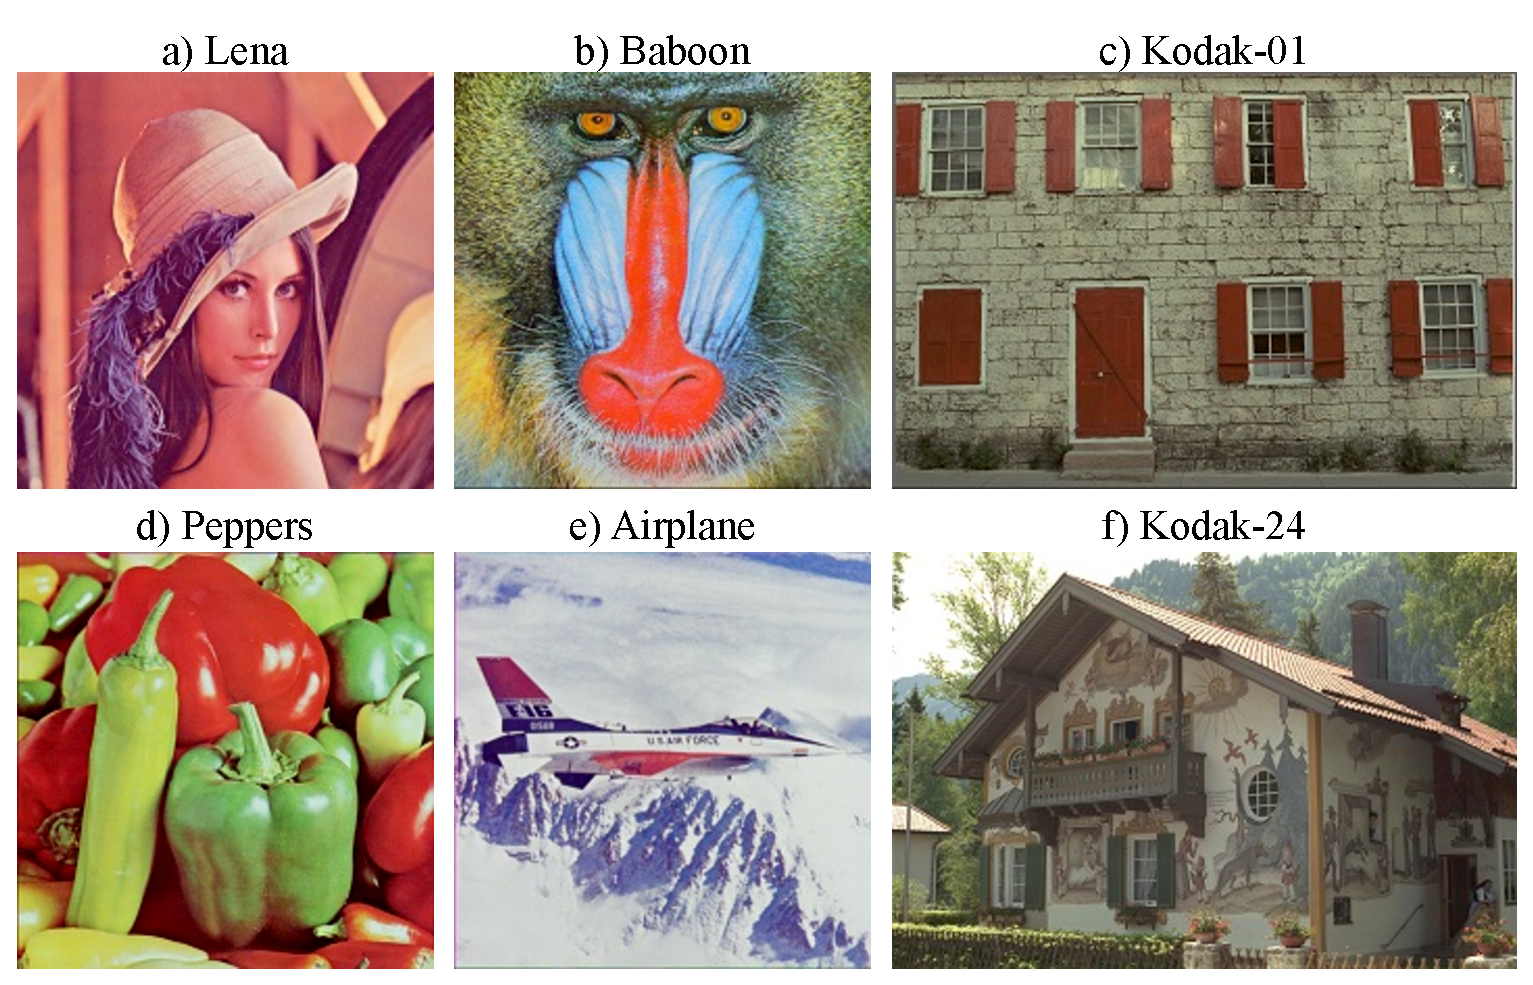
\includegraphics[width=0.9\textwidth]{figures/exp_images.eps}
  \caption{实验用6副彩色图像}
  \label{fig:exp_images}
\end{figure}
\vspace{-7mm}
\par
首先,针对6副彩色图像,我们通过容量-失真曲线研究了提出的算法的性能。容量失真曲
线是一种检验可逆隐藏算法性能的常用手段,以嵌入容量为图像横轴,图像的质量衡量为
纵轴,反映了图像质量同嵌入容量之间的变化关系。在实验中,嵌入容量用嵌入的比特数
表示,图像质量用峰值信噪比(PSNR)来表示。实验用图见图\ref{fig:exp_images},其
中a、b、d、e是$512\times 512$的tiff图像,c、f是两个Kodak图像,大小是$512\times
768$,png格式;6副图像的容量失真曲线如图\ref{fig:6_image_results}。从实验结果
可以看出,本文提出的可逆隐藏算法比文献\cite{li2013reversible}的算法表现更好。
在所有6副图像的结果中,Lena、Baboon、Peppers、Airplane四幅图像的图像质量提升并
不明显,PSNR提升基本都在0.25 dB左右;而Kodak的两幅图像效果提升显著,在2 dB到4 dB
之间。这是由于Kodak两幅图像有较为复杂却规则的纹理,而本文提出的算法能比以往
算法在纹理区域有更好的预测,从而得到更好的实验结果。
\par
随后,我们对UCID数据库超过1300副图像进行了测试,嵌入容量为130000比特,
图\ref{fig:ucid_results}是改进算法图像质量$PSNR_p$同文献\cite{li2013reversible}
算法图像质量$PSNR_{[25]}$的差值直方图。
\begin{figure}[!h]
  \centering 
  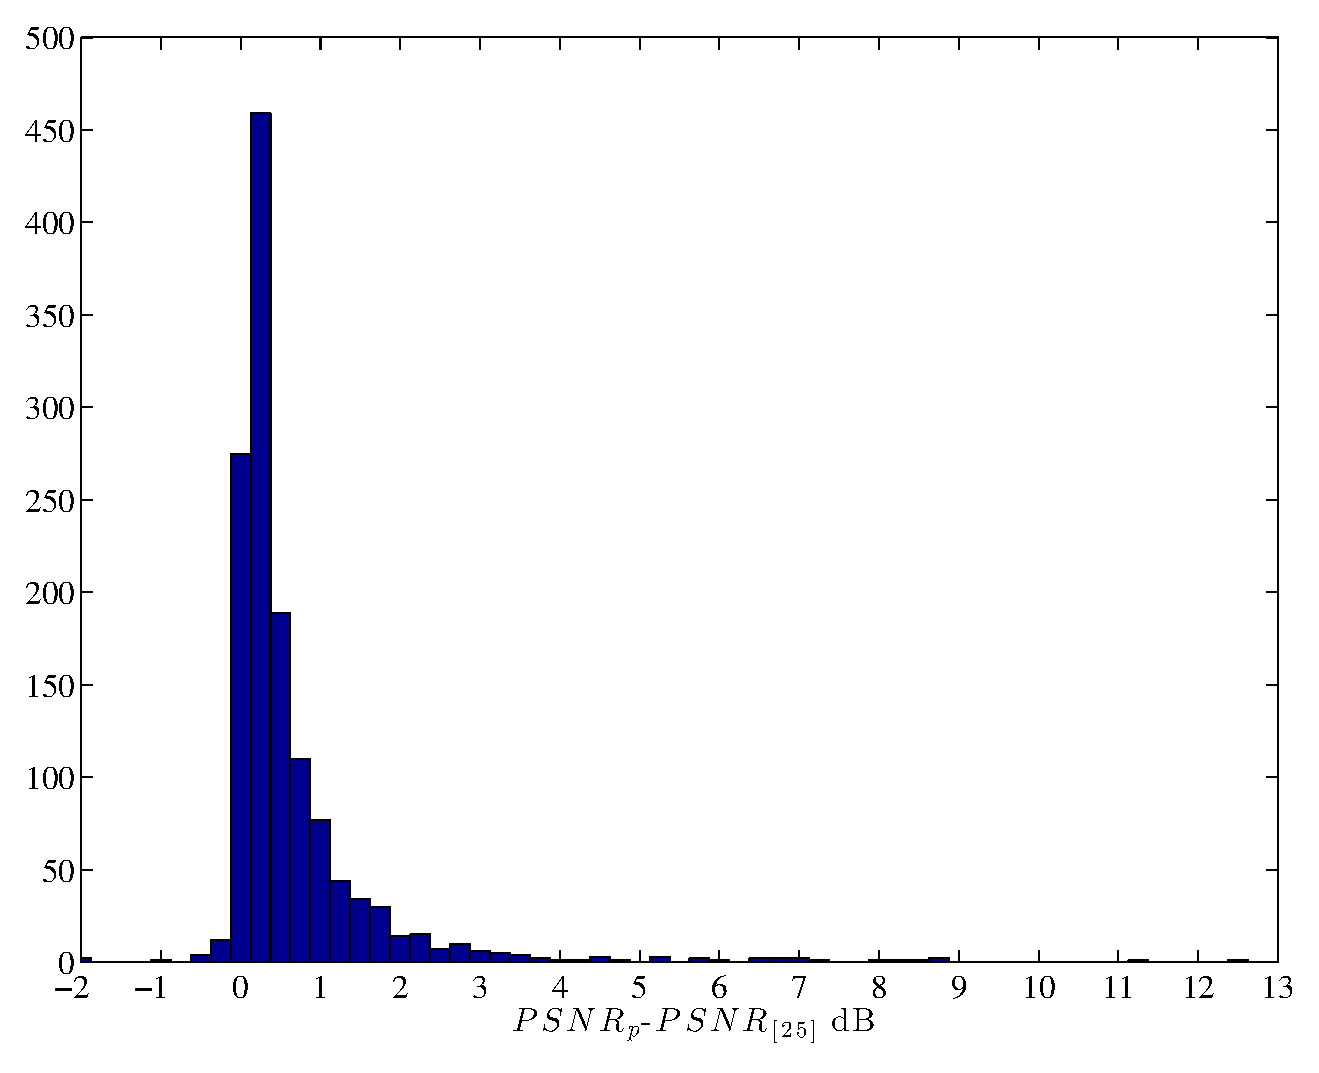
\includegraphics[width=0.9\textwidth]{figures/ucid_results.eps}
  \caption{针对UCID数据库的图像质量提升}
  \label{fig:ucid_results}
\end{figure}
\par
通过图像质量差值我们发现,在超过1000副图像中使用本文提出的算法的图像质量比
使用文献\cite{li2013reversible}的算法图像质量要高,平均PSNR高出0.543 dB,
提升最明显的一幅图像PSNR高出12.474 dB。由此可见,本文提出的算法在绝大多数
情况下都能比文献\cite{li2013reversible}的算法得到更优的结果。
\begin{figure}[!ht]
  \centering 
  \subfigure[Lena]{
    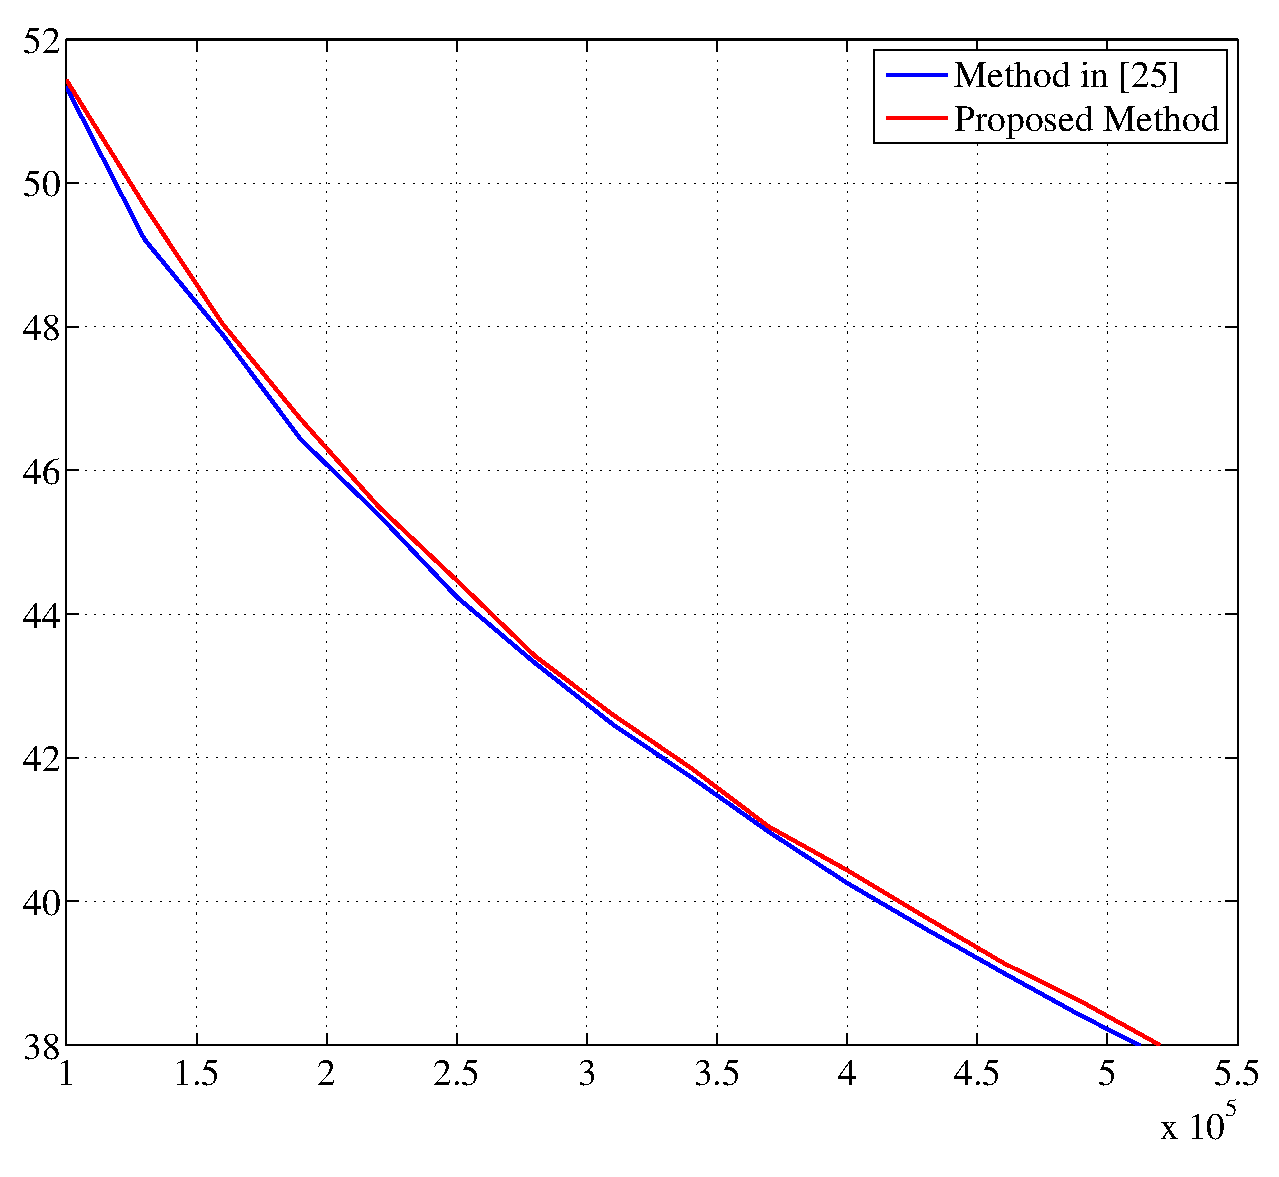
\includegraphics[width=0.4\textwidth]{figures/lena_results.eps}
    \label{fig:lena_results}}
  \subfigure[Baboon]{
    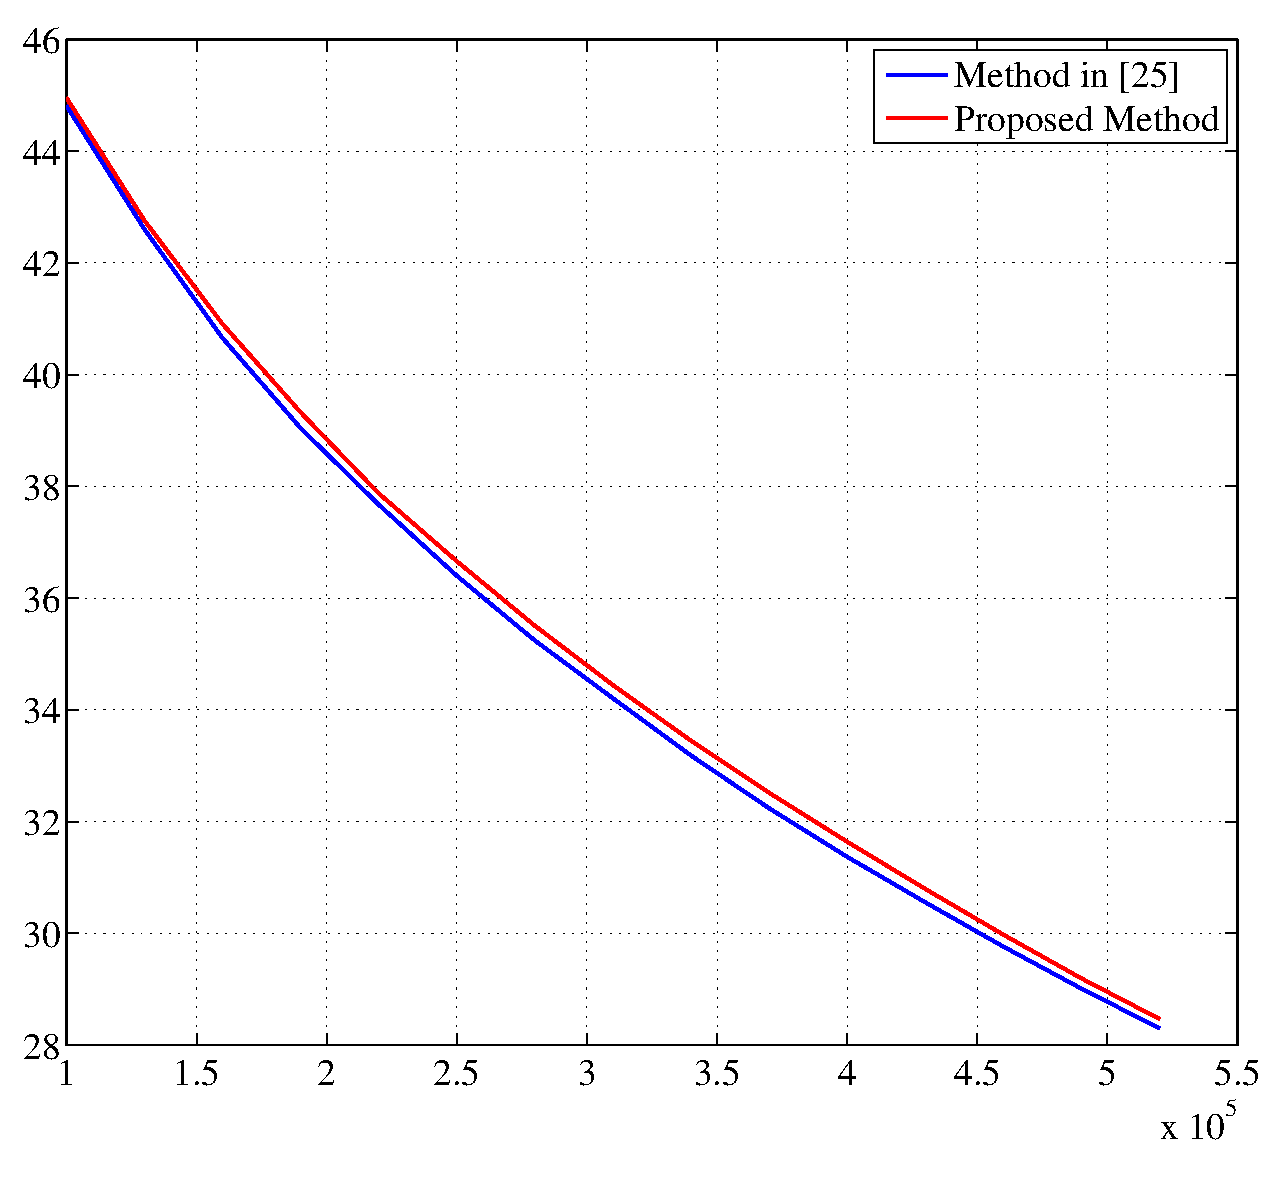
\includegraphics[width=0.4\textwidth]{figures/bab_results.eps}
    \label{fig:lena_results}}\\
  \subfigure[Pepper]{
    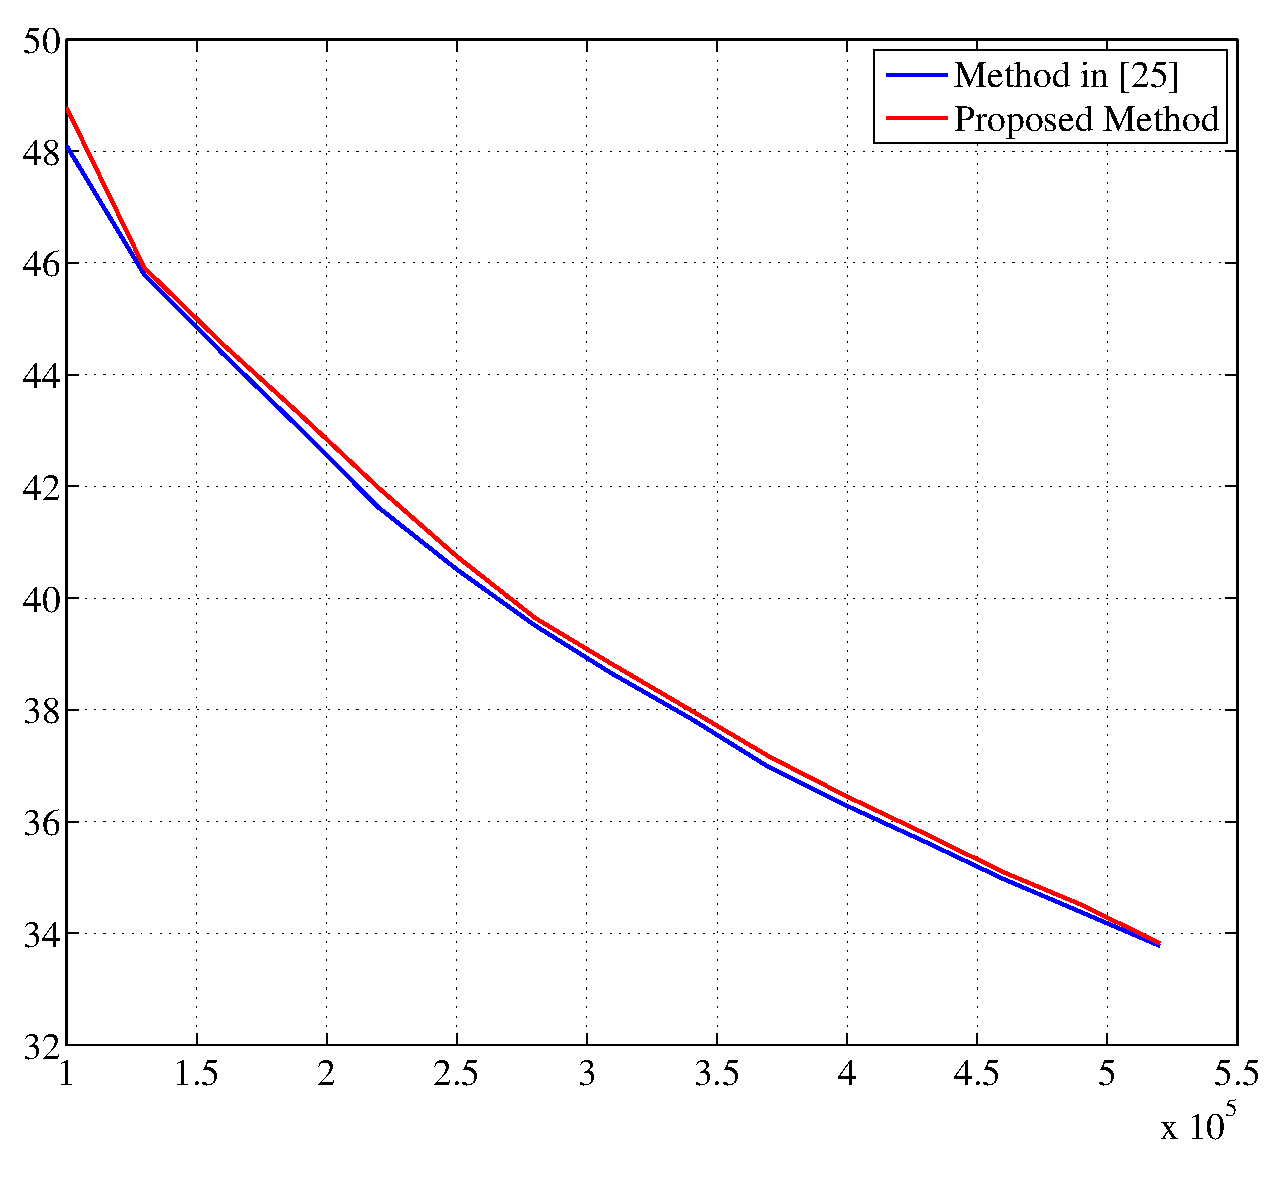
\includegraphics[width=0.4\textwidth]{figures/pep_results.eps}
    \label{fig:lena_results}}
  \subfigure[Airplane]{
    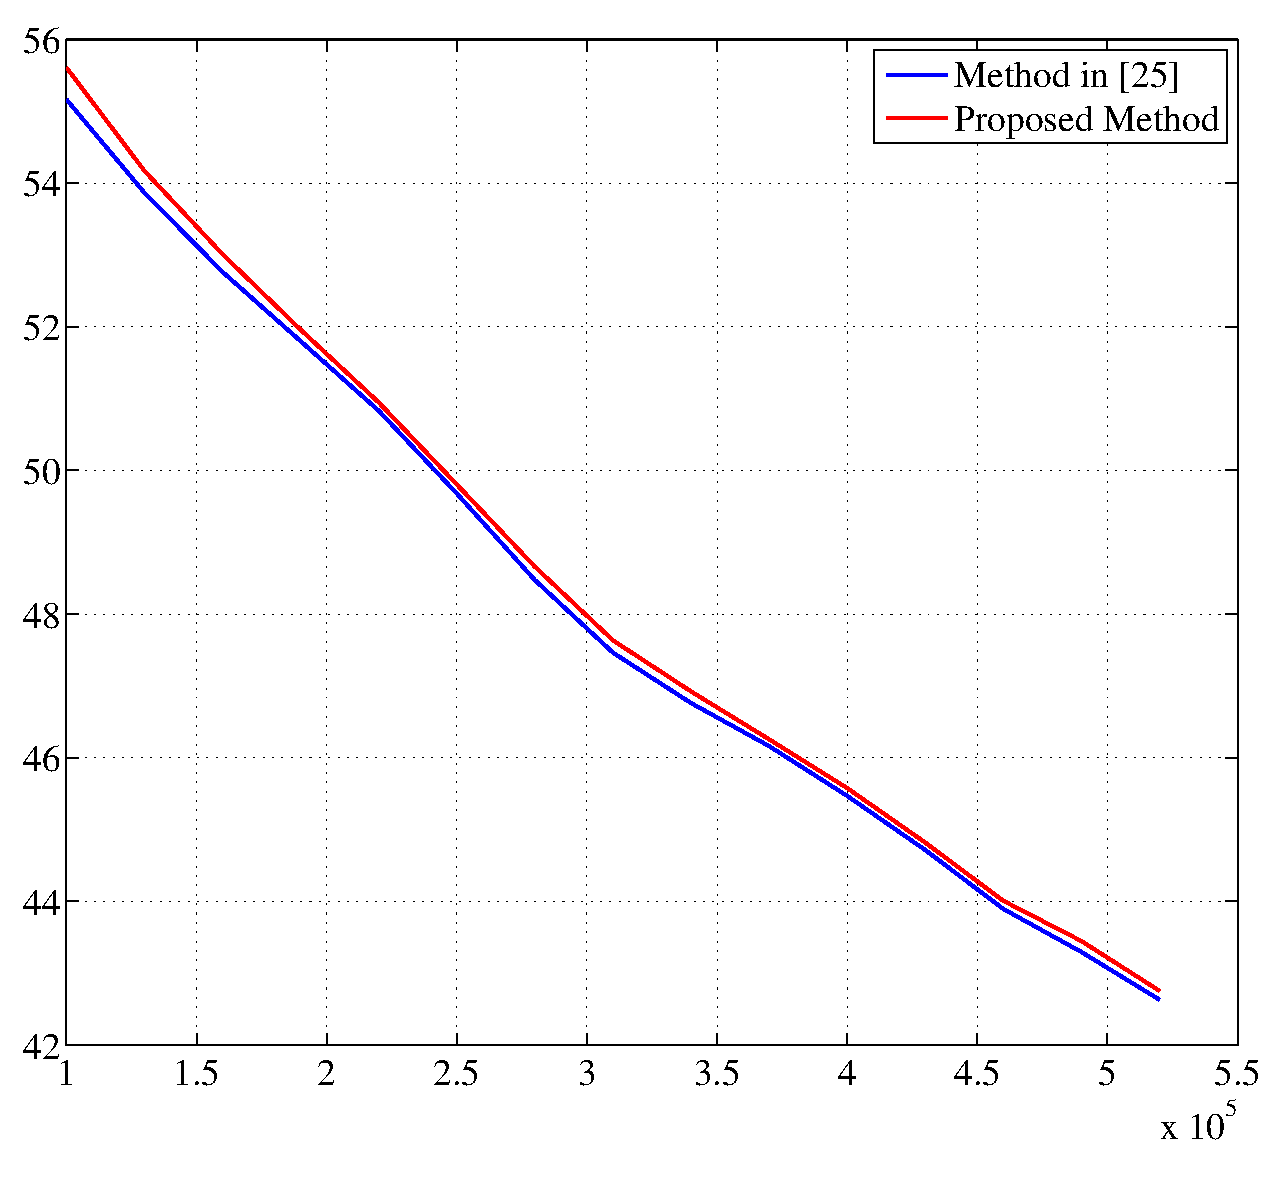
\includegraphics[width=0.4\textwidth]{figures/air_results.eps}
    \label{fig:lena_results}}\\
  \subfigure[Kodak-01]{
    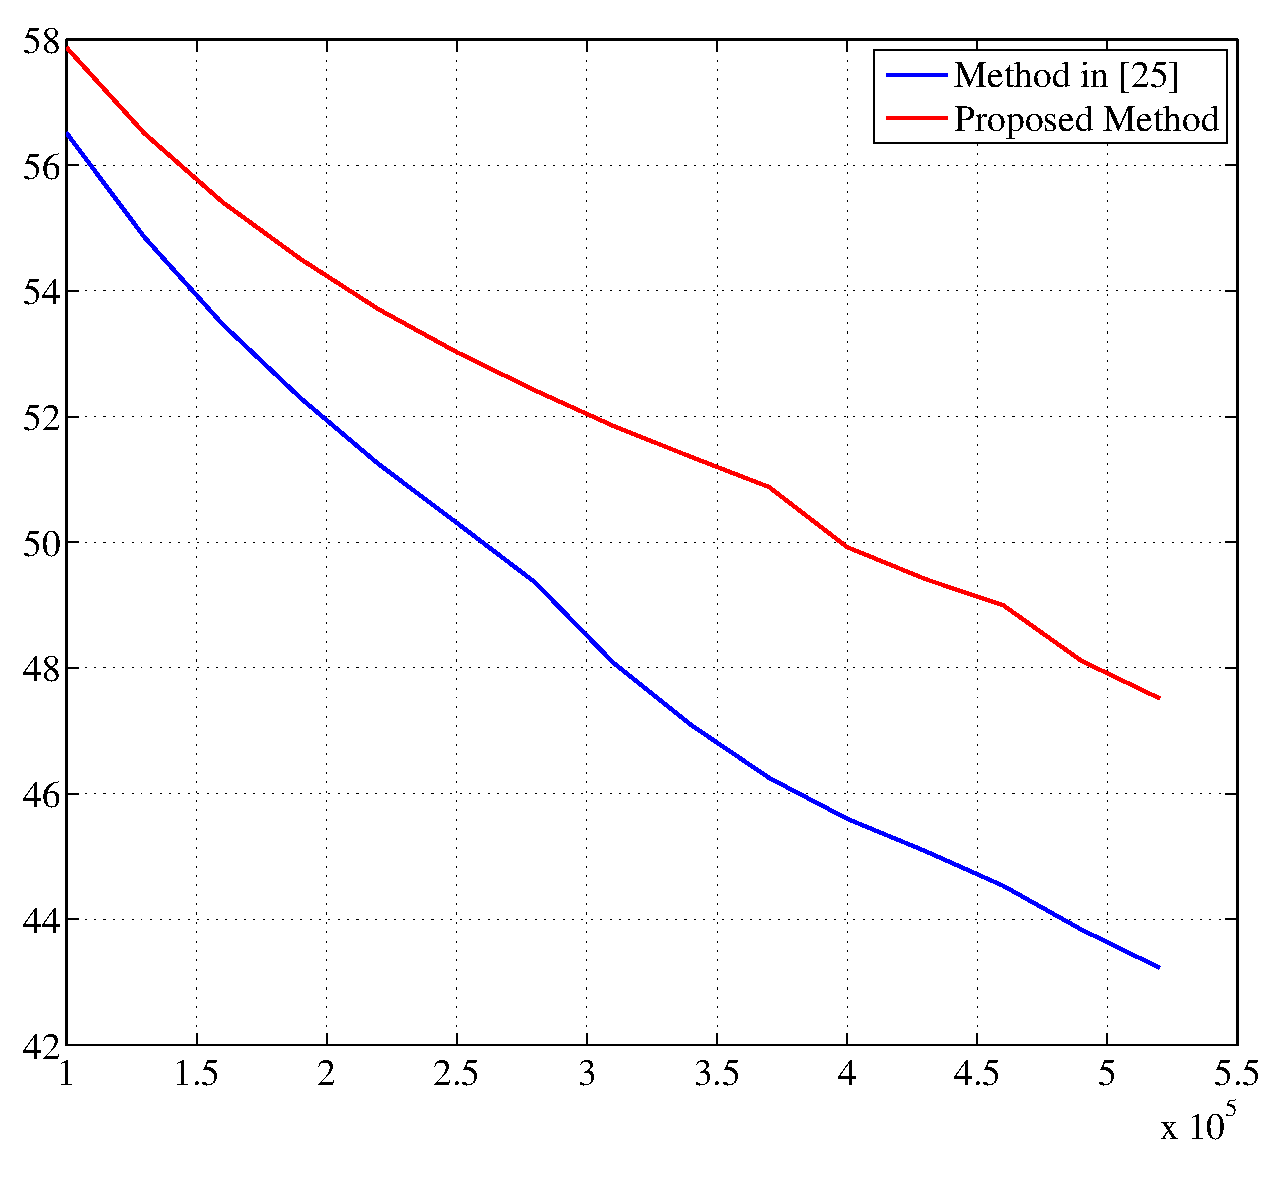
\includegraphics[width=0.4\textwidth]{figures/k1_results.eps}
    \label{fig:lena_results}}
  \subfigure[Kodak-24]{
    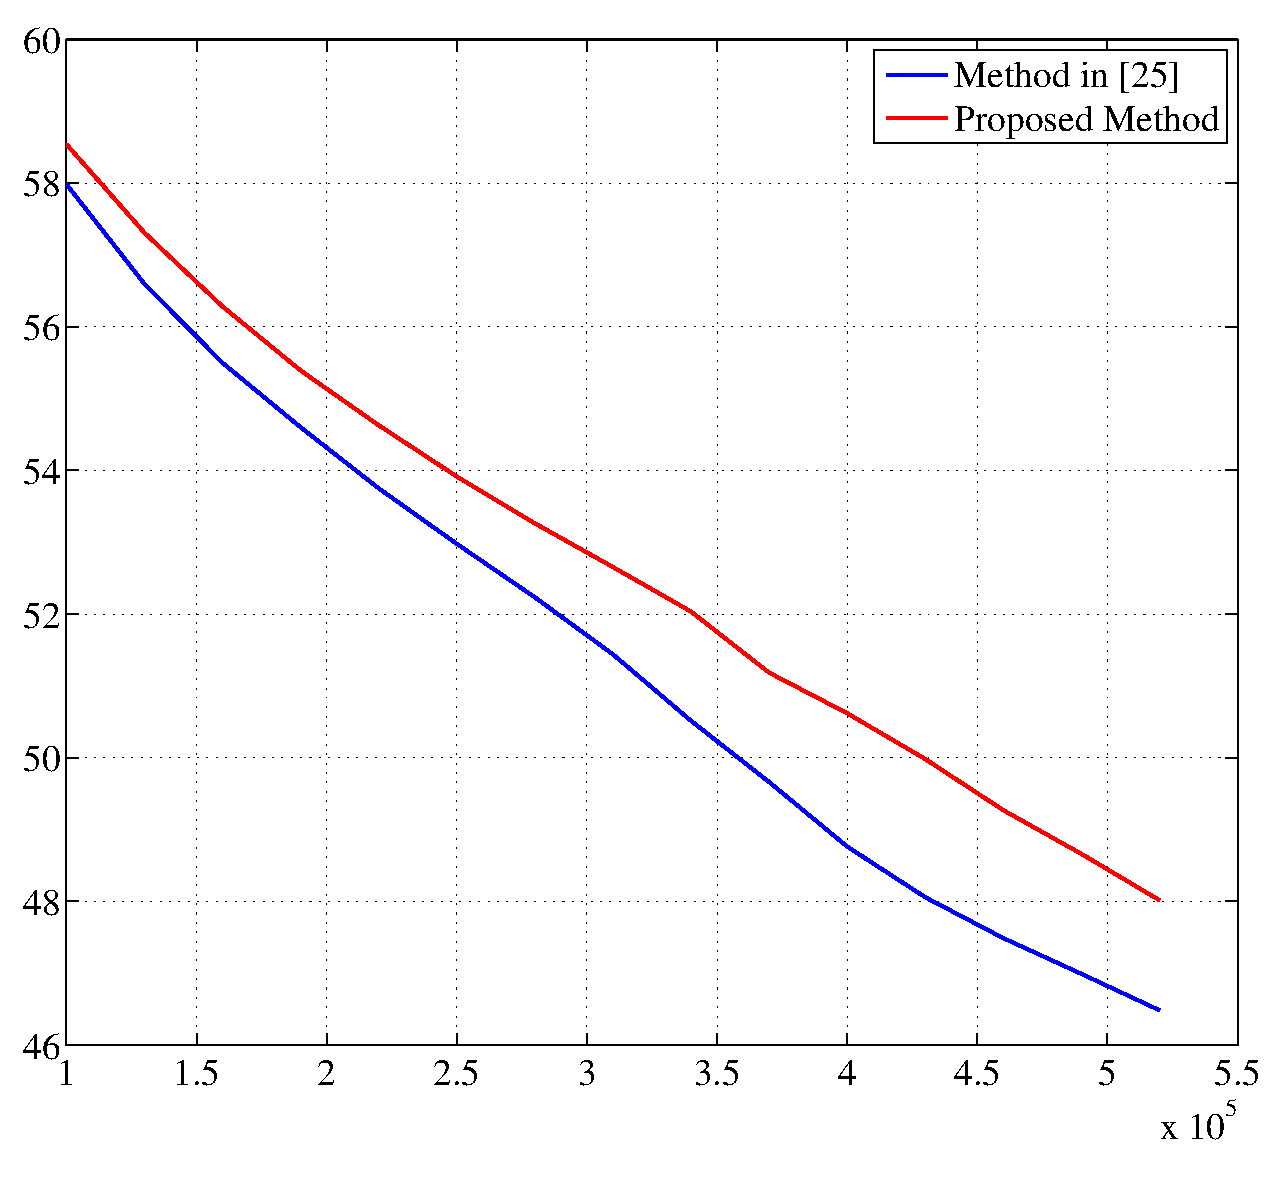
\includegraphics[width=0.4\textwidth]{figures/k2_results.eps}
    \label{fig:lena_results}}\\
  \caption{6副图像的容量失真曲线}
  \label{fig:6_image_results}
\end{figure}

  \chapter{总结和展望}
\label{c:conclusion}

\section{工作总结}
图像的可逆信息隐藏算法在过去几十年中取得了飞速的发展,在可逆隐藏社区出现了诸如基
于可逆压缩的算法,基于扩展的算法,基于整数变换的算法等一批优秀的可逆隐藏算法。其
中基于预测误差扩展的算法是当今应用最广泛,也是最成功的图像可逆隐藏算法,被应用于
灰度图像的可逆隐藏中。但是现阶段的算法大多数只针对灰度图像,而在实际应用中,彩色
图像更为常见。现有的算法当然可以分别应用到彩色图像的三个通道从而实现彩色图像的可
逆隐藏,但是这样并没有充分利用彩色图像本身的通道间的相关性,所以算法仍然有可以改
进的空间。
\par
本文以2013年9月发表在Signal Processing的一篇针对彩色图像可逆隐藏的算法为基础,提
出了一种新的基于彩色图像通道相关性的可逆隐藏算法。在算法中,利用了一种特殊的通道
相关性,即三个通道的图像结构基本相同,纹理复杂度基本相似。这样在三个通道的通道内
进行一轮预测后,三个通道的相同位置的预测值应该是基本相似的。通过通道间进行一轮二
阶预测,可以得到更加准确的预测误差,从而算法的效果得到了提升。
\par
另外,在提出的算法中,使用了一种特殊的针对像素进行排序的算法。传统的像素排序算法
基本都以邻域像素的方差为准则进行排序。而在本文中,排序算法首先对当前像素的预测误
差分布函数进行了预测,然后将分布对y轴取绝对值,将分布函数的峰值同y轴的距离作为像
素预测准确程度的衡量。在文中可以看出,这种排序算法即利用了邻域像素的差值,也利用
到了它们的方差,是一种更加准确的对预测准确程度的衡量。
\par
由实验结果可以看到,文中提出的算法得到了更高的嵌入容量,更好的图像质量,算法成功
的对文献\cite{li2013reversible}进行了改进。

\section{工作展望}
利用彩色图像的通道相关性,进行通道之间的二阶预测方法虽然能得到更为陡峭的、熵更小
的直方图,但是从实验结果中可以看出,最终的改进效果并不明显,针对一副图像,不同嵌
入率下的PSNR的提升只在0.2到0.4之间,提升较小。另外,在相同嵌入率下,对超过1300副
图像的实验结果表明大部分情况下,PSNR的提升在0.25 dB到0.5 dB之间。由此可知,预测
算法对预测性能的提升在实际的隐藏算法中并没有得到充分的利用,究竟如何加以利用需要
更加深入的研究。
\par
针对提升效果微弱这一现象,我们进行了简单地分析。我们认为,反映在预测误差直方图上
的熵的提升,究竟是否如论文中猜测的那样,是在纹理复杂区域由于通道间的二阶预测而导
致的?这一问题需要更加深入细致的对预测过程进行分析,如果并不完全是这样,那么针对
像素的排序算法就需要进一步改进,以针对预测方法的改进,做出适用于该预测方法的排序
算法。
\par
随着可逆信息隐藏技术的不断发展,学者们的目光将陆续集中到针对彩色图像上来。而针对
彩色图像,如何结合彩色图像自身的特点,对其天然的通道间的相关性加以利用,将是可逆
隐藏成功的关键。本本科毕业论文提出了一种简单地利用通道相关性的方法,结合预测误差
扩展的方法,同现有方法相比在嵌入容量和图像质量上有了一定的提升。下一步的工作重点
将是针对所提算法进行进一步的分析,以充分利用预测算法带来的提升;同时如何更好的利
用彩色图像通道间的相关性也是工作的目标。


%%%%%%%%%%%%%%%%%%%%%%%%%%%%%%
%% 附件部分
%%%%%%%%%%%%%%%%%%%%%%%%%%%%%%
%\backmatter

  % 参考文献
  % 使用 BibTeX
  \phantomsection
  \addcontentsline{toc}{chapter}{参考文献}
  \bibliography{bib/tex}
  \nocite{*} % for every item

\end{document}
